\documentclass{article}

\title{EE 371 Autumn 2016 - Lab 3}
\date{\today}
\author{William Li, Dawn Liang, Jun Park}

% general document formatting
\usepackage[margin=1in]{geometry}
\usepackage[document]{ragged2e}
\usepackage{times}

\usepackage{titlesec}
\titleformat{\section}{\Large\bfseries}{\thesection}{0.5em}{\uppercase}

% formatting for code & floats
\usepackage{listings}
\usepackage{color}
\usepackage{graphicx}
\usepackage{float}
\usepackage{wrapfig}

\definecolor{dkgreen}{rgb}{0,0.6,0}
\definecolor{gray}{rgb}{0.5,0.5,0.5}
\definecolor{mauve}{rgb}{0.58,0,0.82}

\lstset{frame=tb,
  language=Verilog,
  aboveskip=3mm,
  belowskip=3mm,
  showstringspaces=false,
  columns=flexible,
  basicstyle={\small\ttfamily},
  numbers=none,
  numberstyle=\tiny\color{gray},
  keywordstyle=\color{blue},
  commentstyle=\color{dkgreen},
  stringstyle=\color{mauve},
  breaklines=true,
  breakatwhitespace=true,
  tabsize=3
}

\begin{document}

% signature page command
\newcommand{\namesigdate}[2][5cm]{
  \begin{tabular}{@{}p{#1}@{}}
    #2 \\[2\normalbaselineskip] \hrule \\[0pt]
    {\small \textit{Signature}} \\[2\normalbaselineskip] \hrule \\[0pt]
    {\small \textit{Date}}
  \end{tabular}
}

\pagenumbering{gobble}
\maketitle
\newpage

\paragraph{Signatures} We certify that the work in this report is our own, and that any work that is not ours is cited.
\paragraph{} \noindent \namesigdate{William Li} \hfill \namesigdate{Dawn Liang} \hfill \namesigdate{Jun Park}

\paragraph{Contributions} William helped with initial hardware design, debugging C code, and the write-up. Dawn wrote the verilog code and tested in iverilog and gtkwave, helped load onto the board and debug with SignalTap, and wrote and compiled the write-up. Jun helped design the system and draw diagrams, wrote verilog code and the C program part of the lab, and helped load onto the board and debug with SignalTap.

\newpage

\tableofcontents
\newpage

\pagenumbering{arabic}

\section{Abstract}
\paragraph{} In this lab, we were tasked with creating a digital 2-scanner system that interacts with a base station to collect underwater data along the canals of Venice. Additionally, we furthered our knowledge of the C programming language by creating two C programs: a temperature conversion program and a digital circuit delay calculator. These projects helped us develop our skills with the various tools and programs used to create both advanced digital designs and complex programs.


\section{Introduction}
\paragraph{} The bulk of the lab focused on our digital design project, a digital continuous 2-scanner system, for retrofitting on gondolas to record valuable underwater environment data along the canal. We worked through the design process by first creating a high-level overview of the system, deciding the necessary modules for the design to work. Next, we decided on the inputs and outputs of each module and the relationships between them. We then built each module in verilog, simulated them in iverilog and gtkwave, uploaded our complete design into Quartus and tested on the DE1-SoC, and used SignalTap II to probe our design and detect errors. Finally, we furthered our knowledge of the C language by writing making two programs: a temperature conversion program and a digital circuit delay calculator. 


\section{Discussion}
\subsection{Design}
  \subsubsection{Design Specification}
  \paragraph{VHDL} The continuous 2-scanner system must constantly be scanning the underwater environment. It does so by trading off scanning and transferring/flushing between the two scanners. Each scanner emits a signal telling the home base that it is ready to transfer as its data buffer reaches 50\% full. When a scanner’s buffer reaches 80\% full, it wakes up the other scanner, and at 90\% it signals the other scanner to start scanning. At 100\%, it enters the idle state, where it waits for a signal to let it begin transferring data, or it is told to flush out its buffer by the other scanner as it reaches 50\%. It takes at least half as long to flush or transfer data as it does to acquire; each scanner must also flush data quickly enough that it is ready by the time the other scanner issues a command.

  \paragraph{C Program} The temperature conversion program is required to take an input and output temperature scale (F, C, or K) and an input temperature value, and output the temperature converted into F, C, and K. The gate delay calculator must take the number of gates in a signal path as input, and output the total gate delay in that path. As an extra feature, both programs prompt the user for a new input if the user inputs an invalid value. The re-prompt message explains why the earlier input was invalid so that the user can correct their mistake.

  
  \subsubsection{Design Procedure}
  \paragraph{VHDL} The main components of the digital scanning system are the two scanners. Each scanner consists of a control system and a memory system. The control system cycles through various states: low power, standby, scanning, idle, transferring, and flushing. Thus, we used an FSM to model it. The memory system was implemented using a basic counter, the value of which indicated the percent full of the data buffer. To model different speeds for scanning, transferring, and flushing, we made various clock speeds that connected to the counter depending on the current state of the scanner. The overall scanner module handled the scanner’s input/output signals, such as the signal indicating that it is ready to transfer and the signals communicating with the second scanner.

  \paragraph{C Program} For temperature.c we first had to understand the equations to convert from one scale to another. The following equations were used:
    \lstinline{tempC = (tempF-32.0) * (5.0/9.0);} and \lstinline{tempK = tempC + 273.15;}

  \paragraph{} For calculateDelay.c we had to include the delay introduced by the trace in calculating the total delay by using this equation:
    \lstinline{totalDelay = gates*5000 + (gates-1)*18;}
  The totalDelay is in units of picoseconds, and this was converted to nanoseconds before being displayed to the user for easy viewing. 

  \paragraph{} After discovering that it was very easy to input an invalid value, we decided to include a way to capture invalid user inputs. In case, by re-prompting the user. For example, inputting a string instead of an integer when the program is expecting an integer should not crash the program, but instead cause the program to re-prompt.


  \subsubsection{System Description}
  \paragraph{VHDL} The digital scanning system continuously collects data from the underwater environment by cycling between two scanners.

  \paragraph{Inputs to the system}
  \paragraph{} User inputs
  \begin{itemize}
    \item reset: the system resets to be inactive, so both scanners are in the low power state and the data buffer is clear
    \begin{itemize}
      \item SA0: the system will never reset to known values at startup, so it cannot begin normal operation
      \item SA1: the system will be in constant reset mode
    \end{itemize}

    \item initialOn: the system is initially inactive. It switches on and begins scanning when it receives an initial ‘on’ signal, at which point in begins continuously scanning and cycling between the two scanners.
    \begin{itemize}
      \item SA0: the system will never turn on initially, so it will never begin scanning
      \item SA1: the system will always be on; upon reset, the system will not become inactive but rather begin scanning immediately, and otherwise operate normally
    \end{itemize}

    \item startTransfer: once the scanners have reached 100\% (data buffer full), they must wait for a signal from the base station in order to transfer data
    \begin{itemize}
      \item SA0: the scanners will never transfer data, always flushing it out
      \item SA1: the scanners will always transfer their data, never flushing
    \end{itemize}
  \end{itemize}

  \paragraph{Outputs of major functions}
  \paragraph{} Communication between the scanners
  \begin{itemize}
    \item goToStandby: when one scanner reaches 80\%, it issues a goToStandby signal to the other scanner, telling it to wake up and prepare to scan
    \begin{itemize}
      \item SA0: the scanners will not tell each other to wake up, so there will not be continuous cycling of scanning
      \item SA1: the scanners will immediately go to standby mode once they finish flushing/transferring, otherwise operating normally
    \end{itemize}

    \item startScan: when one scanner reaches 90\%, it issues a startScan signal to the other scanner, telling it to begin scanning and collecting data
    \begin{itemize}
      \item SA0: the scanners will not tell each other to start scanning, so there will not be continuous cycling of scanning
      \item SA1: the scanners will immediately start scanning once they have gone to standby mode, otherwise operating normally
    \end{itemize}

    \item flush: when one scanner reaches 50\%, it sends a flush signal to the other scanner. if the other scanner is at 100\% (has not transferred its data), it will empty its data buffer.
    \begin{itemize}
      \item SA0: the scanners will not tell each other to flush, so they will remain in idle until they receive a startTransfer signal, breaking the continuous scanning cycle
      \item SA1: the scanners will always flush their data once they reach the idle state, never tranferring to the base station
    \end{itemize}
  \end{itemize}
  
  \paragraph{} Overall scanner system
  \begin{itemize}
    \item readyToTransfer: when a scanner reaches 50\%, it sends a readyToTransfer signal to the base station.
    \begin{itemize}
      \item SA0: the base station will never think the scanner is ready to transfer, so it will never issue a startTransfer signal and the scanner system will never tranfer its data (always flush)
      \item SA1: the base station will think the scanner is always ready to transfer, so it will constantly issue a startTransfer signal; otherwise, the system operates normally
    \end{itemize}

    \item Scanner states \& progress: each scanner outputs which state it is currently in and its buffer fill percentage
    \begin{itemize}
      \item if any of these values fault, the scanner will break fatally
    \end{itemize}
  \end{itemize}

  \begin{figure}[H]
    \centering
    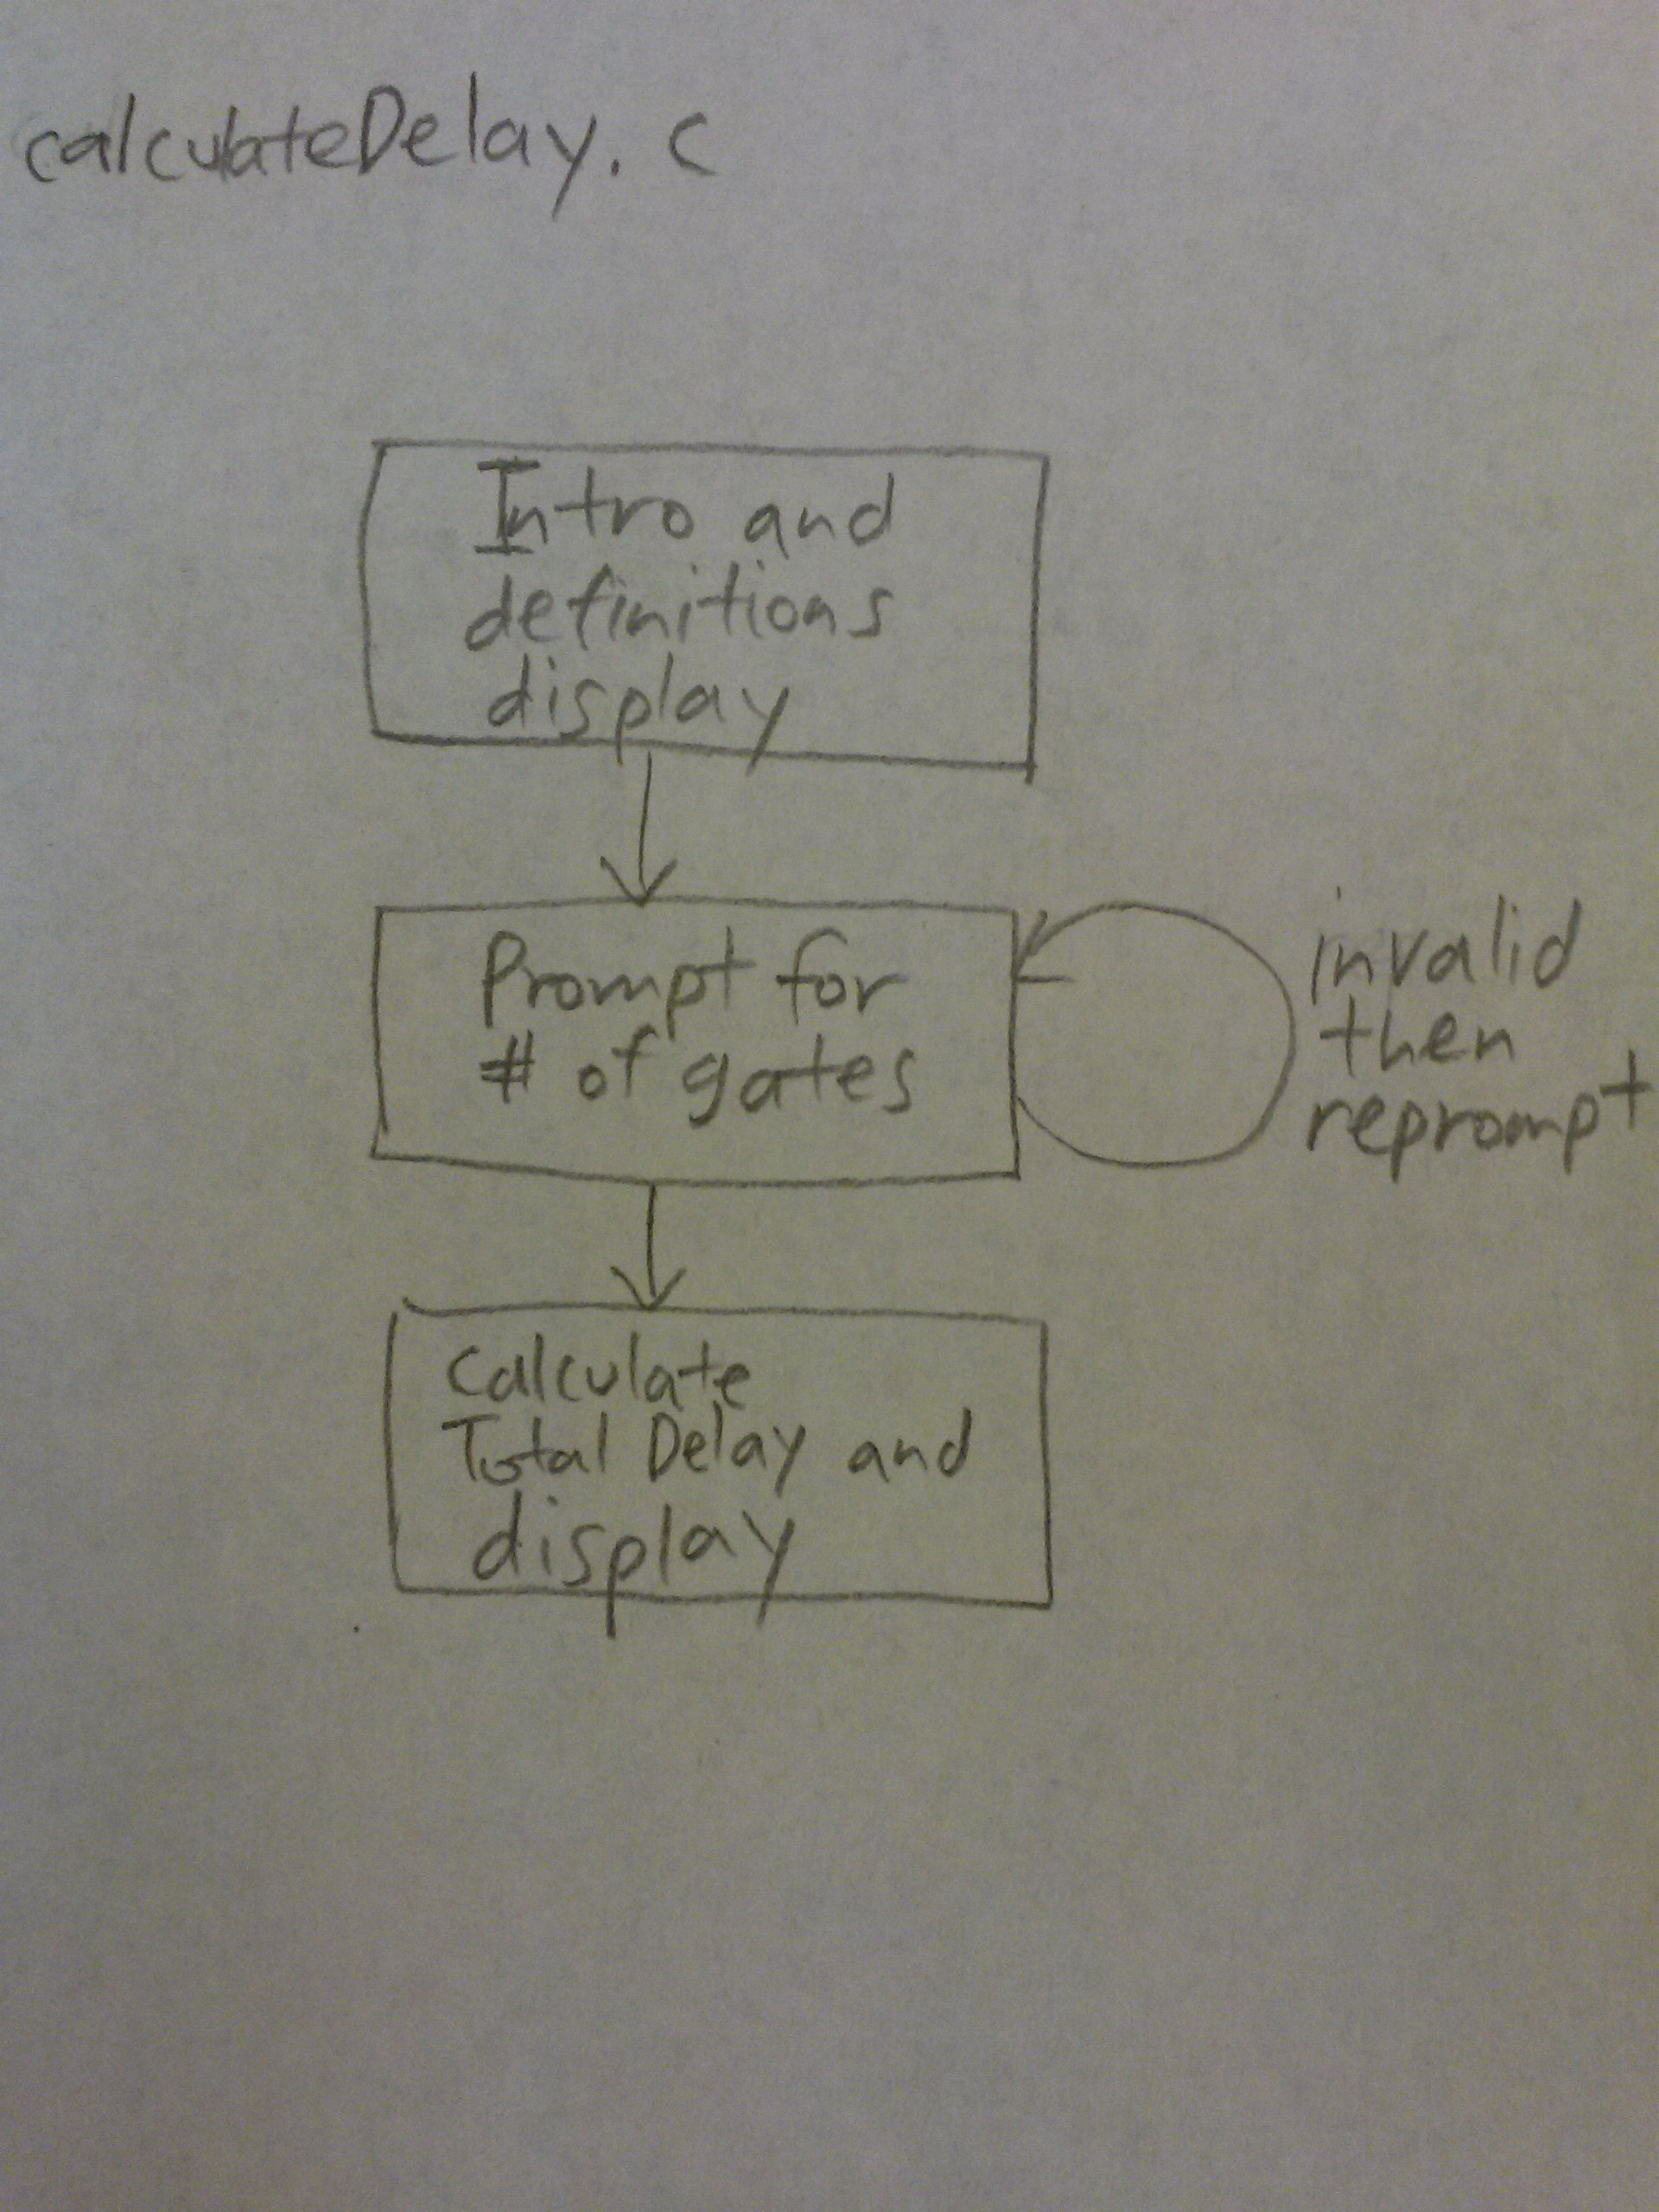
\includegraphics[width=0.75\linewidth]{figures/c/calcDelay_blockdiagram.jpg}
    \caption{Block diagram of calcDelay.c program}
    \label{fig:calcDelay_blockdiagram}
  \end{figure}

  \begin{figure}[H]
    \centering
    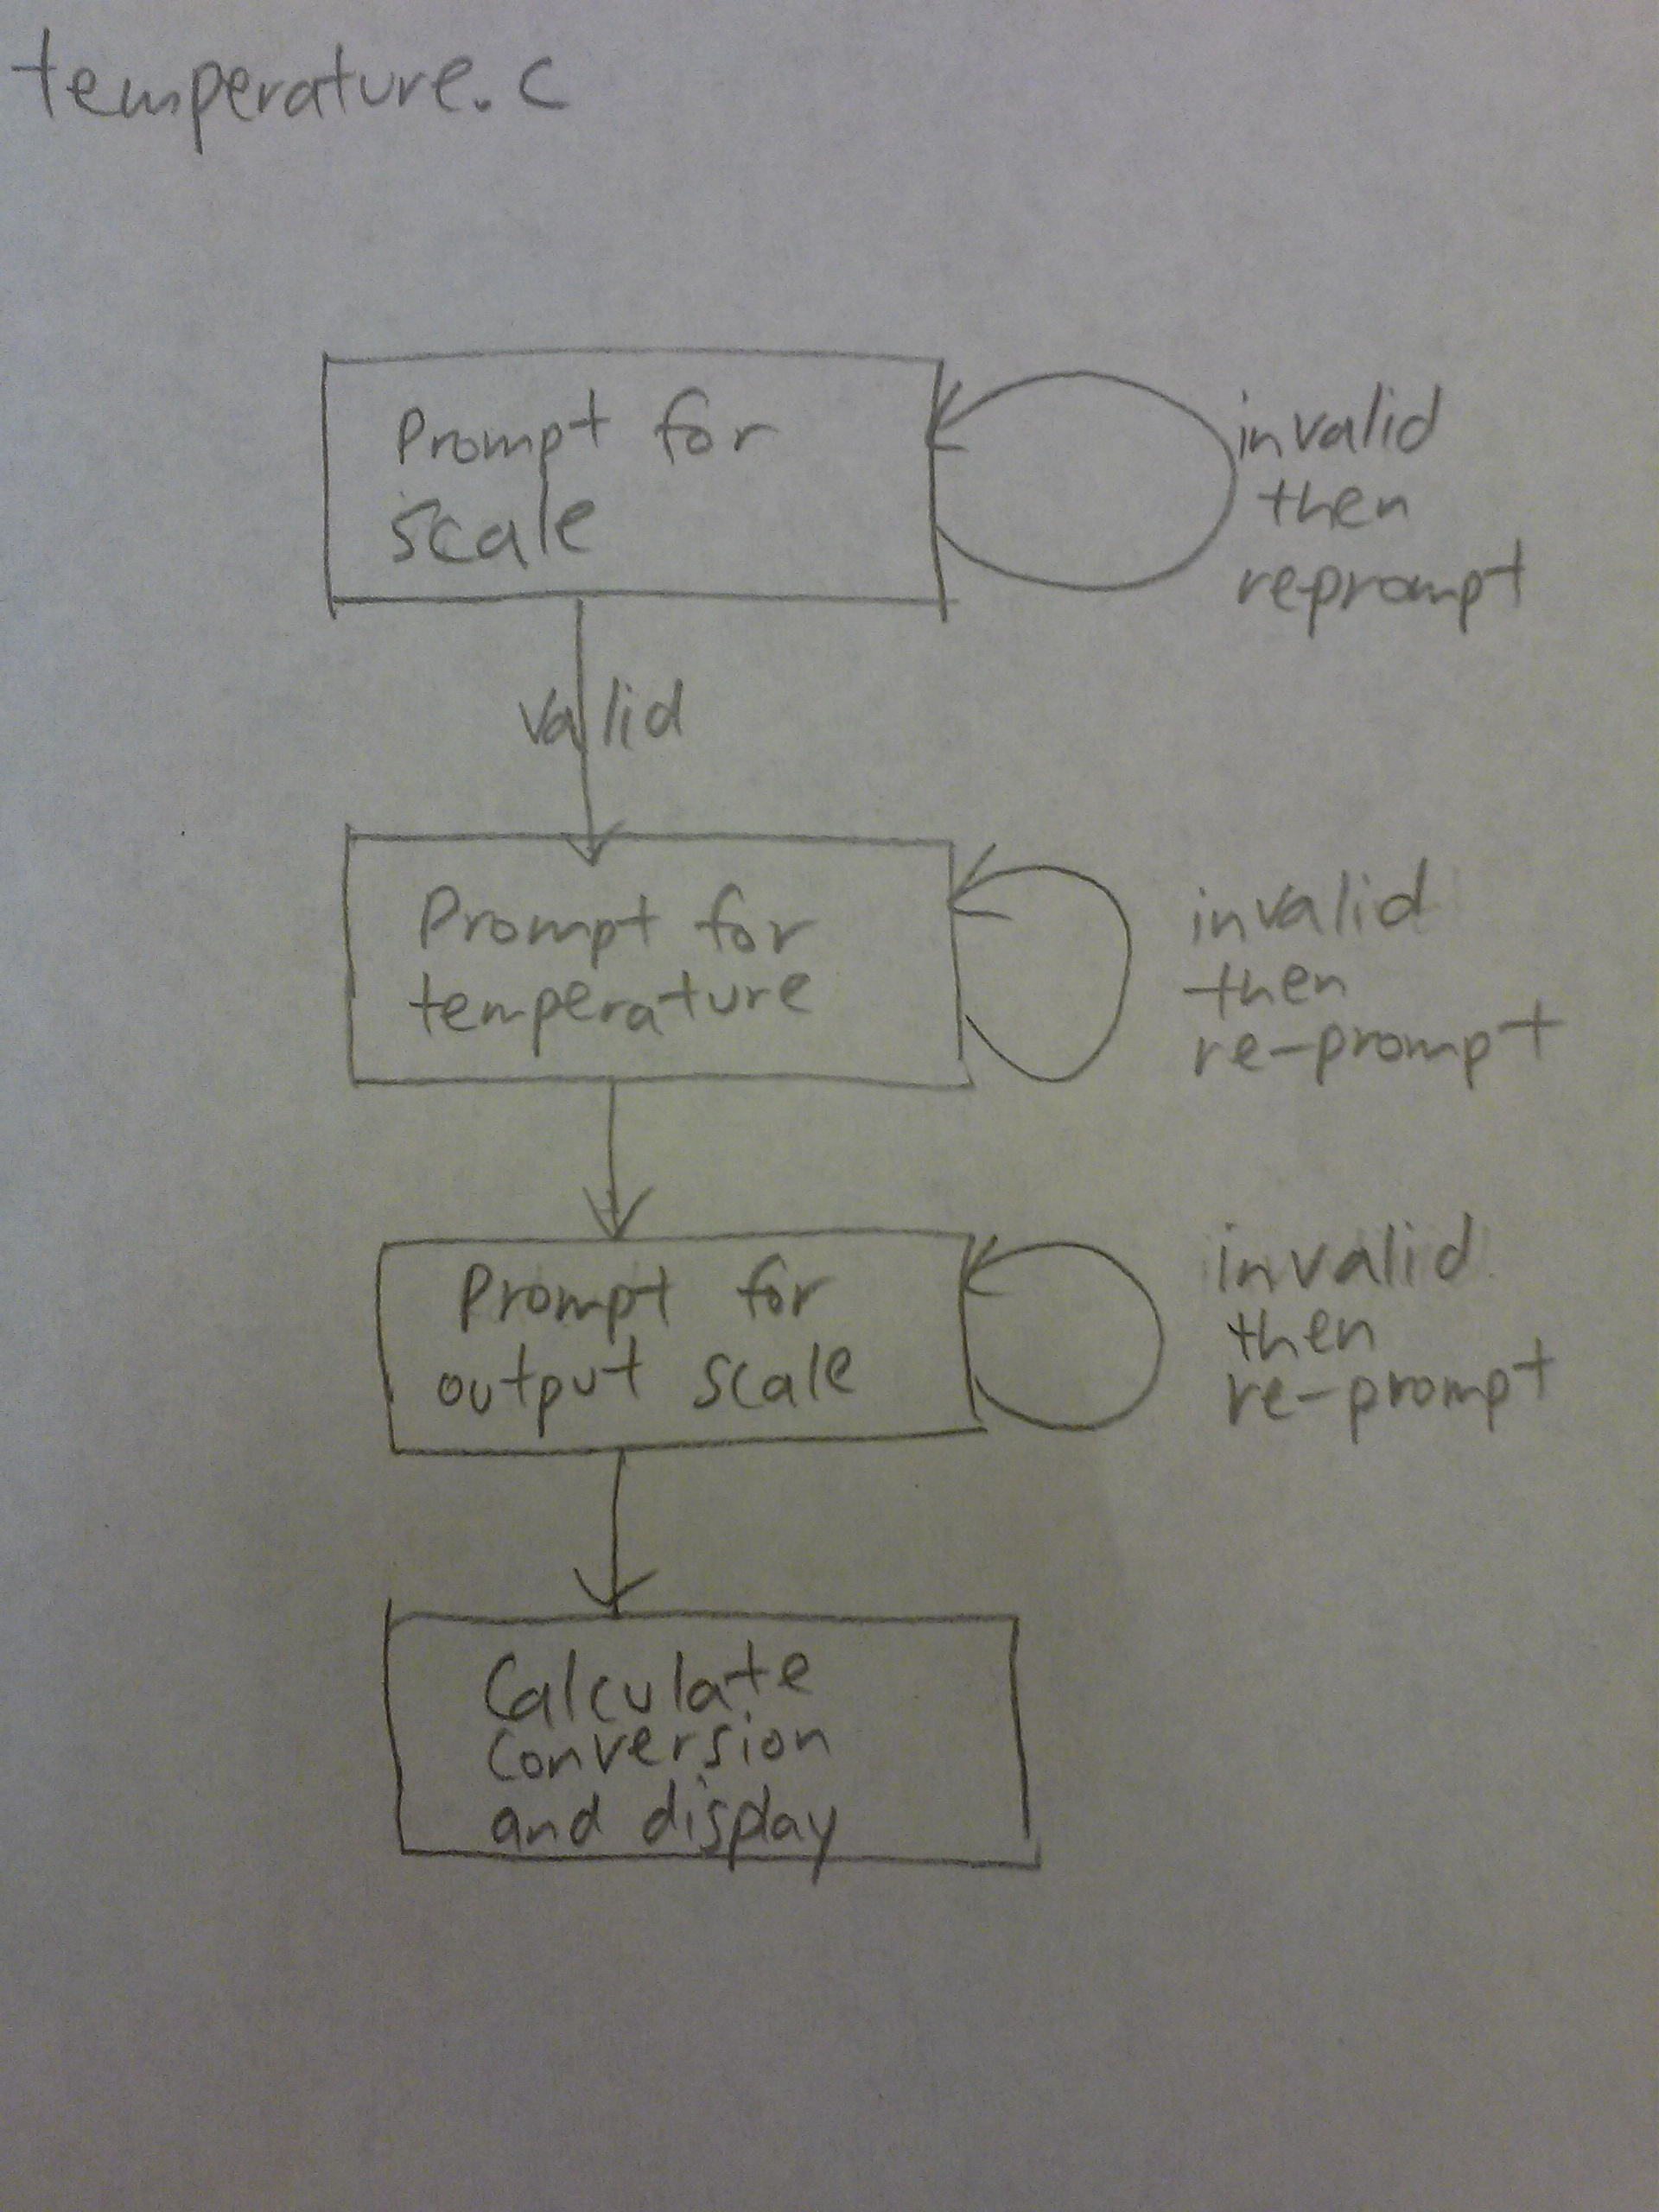
\includegraphics[width=0.75\linewidth]{figures/c/temp_blockdiagram.jpg}
    \caption{Block diagram of temperature.c program}
    \label{fig:temp_blockdiagram}
  \end{figure}


  \subsubsection{Software Implementation}
  \paragraph{} The temperature.c program prompts the user for a temperature scale, the temperature, and a temperature scale to convert to. The program then converts and displays the temperature in the scale requested by the user. The program re-prompts the user if the user inputs an invalid temperature scale. The program also re-prompts if the user inputs an invalid temperature. When a valid scale and a valid temperature is input by the user, the program prompts for a temperature scale to convert to. The program re-prompts the user if the user inputs an invalid scale. Once all user inputs are correct, the program converts the temperature and displays the result.

  \paragraph{} The calculateDelay.c program prompts the user for the number of logic gates in a signal path, then calculates and displays the total delay along that path both in picoseconds and nanoseconds. The program re-prompts the user if the user inputs an invalid number of gates. The program also displays a definition of how the total delay is calculated upon startup.


  \subsubsection{Hardware Implementation}
  \paragraph{} The digital scanner contains two scanners that transfer data to a base station and alternate in scanning cycles. They communicate with the base station to transfer data, and communicate with each other to indicate when to wake up, start scanning, or flush data.

  \paragraph{} Each scanner has a control system and a memory system.

  \paragraph{} The control system determines the scanner’s state: low power, standby, scanning, idle, transferring, or flushing. Based on input signals from the other scanner and from base station, as well as the current buffer percentage, the control system transitions the scanner between these states.

  \paragraph{} The state of the scanner then determines the behaviour of the memory system - whether it is collecting data, holding, or transferring/flushing data. Since collecting data must take at least twice as long as transferring/flushing data, the memory system must also be modeled using variable clock speeds. We did this using a counter that connected to a different speed clock depending on the scanner’s state.

  \paragraph{} The scanner outputs various signals to communicate both with the other scanner and the base station, as well as display its current state and progress. These signals are implemented through combinational logic, as they occur when the scanner’s buffer has reached a specific percentage in the scanning state (i.e. \lstinline{out = (buffer == percentage && state == desiredState)}).

  \paragraph{} For viewing on the DE1-SoC, each scanner’s state and progress are displayed on three HEX displays per scanner, and the 1-bit output signals are displayed using LEDs. The user input signals (reset, initialOn, and startTransfer) are assigned to KEYs and SWs, to model base station signals or turning the system on initially.

\subsection{Test}
  \subsubsection{Test Plan}
  \paragraph{VHDL} The digital scanner system was tested under normal operating conditions: it should begin scanning when prompted. Upon reaching 50\%, it must issue a readyToTransfer signal as well as a signal for the other scanner to flush. At 80\%, it should wake up the other scanner, and at 90\% it should tell the other scanner to start scanning. At 100\%, the scanner should enter the idle state, where it waits for either a startTransfer signal from the base station or a flush signal from the other scanner, whichever comes first. It should then enter the lowPower state, and go to standby and begin scanning at the prompting of the other scanner. As a detail, it is important that each scanner flushes quickly enough (when the other scanner reaches 50\%) that it is ready to go to standby when the other scanner prompts it to (at 80\%).

  \paragraph{} There were relatively few inputs, so failure conditions were few. Of these, we tested that the system only transferred once at 100\% in the idle state (did not transfer if it received the signal while not idle), that it issued the output/scanner communication signals only while scanning, and what occurred when the scanner received both the startTransfer and flush signal at the same time. Finally, the reset input should put the system in the reset state.

  \paragraph{C Program} The temperature.c program needs to be run with the various temperature scale and temperature inputs to make sure it is outputting the correctly converted value to the correct output scale. The calculateDelay.c program needs to be run with various gate number inputs to make sure it is outputting the correct Total Delay time both in picoseconds and nanoseconds. Both temperature.c and calculateDelay.c need to be tested with non valid inputs to ensure they are properly handling invalid inputs with a re-prompt to the user.


  \subsubsection{Test Specification}
  \paragraph{VHDL} The primary outputs of the two-scanner system, the state and data buffer percentage of each scanner, were monitored. Additionally, each individual scanner’s output signals for communication between the scanners were monitored. As there were only three inputs, it was relatively simple to test the system constraints.

  \paragraph{} The scanner should transition through the states in order, as depicted in the state diagram (see state transition diagram). Additionally, it should be filling the data buffer (increasing percentage) in the scanning state, and emptying the data buffer (decreasing percentage) in the transferring and flushing states. The data buffer should empty at least twice as fast as it fills, and for flushing, it should empty by the time the other scanner reaches 80\% and sends a goToStandby signal. On reset, the scanner should go to the lowPower state and the data buffer should go to 0\%.

  \paragraph{} Each scanner’s communication signals should only output when in the scanning state (e.g. it should not issue a readyToTransfer signal when it reaches 50\% while flushing). Additionally, the signals should become active at the correct percentage of data buffer full: 50\% for readyToTransfer and otherFlush, 80\% for otherGoToStandby, and 90\% for otherStartScan.

  \paragraph{C Program} The temperature.c program needs to be tested with various input temperature scales, temperature inputs, and output temperature scales to ensure that it is converting the temperatures correctly and according to the scale specified by the user. For example, inputs: F, 32, C should output 0 degrees on the Celsius scale. 

  \paragraph{} The calculateDelay.c program needs to be tested with various integer inputs to ensure it is calculating the total path delay correctly while following the definitions  that: each gate has a 5ns delay, 1in of trace has a delay of 180ps, and that the output of one device to the input of the next device is connected by 0.1in of trace.  For example, input of 5 should output 25072ps and 25.072ns. 

  \paragraph{} Both programs need to be tested with likely invalid user inputs to make sure the programs are handling the invalid inputs with a correct re-prompt. For example, inputting a non valid scale like j into temperature.c should cause it to re-prompt for a valid scale, while inputting a non valid gate number like 4.3 into calculateDelay.c should cause it to re-prompt for a valid gate number.


  \subsubsection{Test Cases}
  \paragraph{VHDL}

  \paragraph{} Pass cases
  \begin{itemize}
    \item Reset case
    \begin{itemize}
      \item Input: reset = 1
      \item Measure: state and data buffer
      \item Pass condition: state = lowPower, data\_buffer = 0 (lowPower mode and empty data buffer)
    \end{itemize}

    \item turning on the scanner system
    \begin{itemize}
      \item Input: initialOn = 1
      \item Measure: states of each scanner
      \item Pass condition: one scanner should be in scanning mode, and the other should be in lowPower mode
    \end{itemize}

    \item transferring data
    \begin{itemize}
      \item Input: startTransfer = 1
      \item Measure: state of the scanner
      \item Pass condition: if idle, the scanner should go to transferring mode. Otherwise, the scanner should hold its state
    \end{itemize}
  \end{itemize}

  \paragraph{} Fail cases
  \begin{itemize}
    \item transferring while not on
    \begin{itemize}
      \item Input: initialOn = 0, startTransfer = 1
      \item Measure: state of the scanner
      \item Pass condition: nothing should happen, as the scanners haven’t been turned on yet
    \end{itemize}

    \item transferring while not in the idle state
    \begin{itemize}
      \item Input: startTransfer = 1 while not in the idle state
      \item Measure: state of the scanner
      \item Pass condition: nothing should happen, since the scanner isn’t in the idle state
    \end{itemize}

    \item simultaneous startTransfer and flush signals
    \begin{itemize}
      \item Input: startTransfer = 1 \& flush = 1
      \item Measure: state of the scanner
      \item Pass condition: the scanner should prioritise transferring over flushing, so it should go to the transferring state
    \end{itemize}
  \end{itemize}

  \paragraph{C Program}
  \begin{itemize}
    \item Address all compiler errors then compile and run temperature.c and calculateDelay.c.
    \item Valid temperature scale inputs for temperature.c are: f, F, c, C, k, K where each character represents Fahrenheit, Celsius, or Kelvins. Try each of these inputs. 
    \item Valid gate number input for calculateDelay.c are non-negative integers. For example, you can’t have half a gate, nor a negative number of gates. Try the valid inputs (non-negative integers) first. 
    \item temperature.c should output a correctly converted decimal value representing the temperature in the specified scale rounded to two decimal places. 
    \item calculateDelay.c should output a correctly calculated Total Delay and output that value in both picoseconds and nanoseconds. 
    \item For both programs, intentionally input an invalid value and make sure that the program re-prompts instead of crashing or giving an incorrect value. For example, inputting a string when an integer or double is expected by the program and observing what the program does.
  \end{itemize}


\section{Results}
  \paragraph{VHDL} The digital scanning system performed as expected under normal operating conditions and under edge and fail cases.

  \paragraph{} When the system is reset, it goes to the expected reset state (lowPower \& 0\% buffer). Nothing happens until it is turned on (initialOn = 1), at which point one scanner begins scanning while the other stays in lowPower. When the first scanner reaches 50\%, it issues a readyToTransfer signal to the base station and a flush signal to the other scanner. When it reaches 80\%, it wakes up the other scanner, and at 90\% it tells the other scanner to begin scanning. At 100\%, it goes into the idle state while the other scanner is scanning, and waits for a startTransfer signal from the base station or a flush signal from the other scanner, whichever comes first. It transfers data/flushes accordingly, then goes to the lowPower state and waits to be woken up by the other scanner. The scanners trade off and cycle through these states accordingly, so that there is always at least one scanner scanning at all times.

  \paragraph{} If a scanner is given an input before it has been turned on, it doesn’t do anything, as expected. Additionally, each scanner only transfers once it has reached the idle state; it does not transfer until it has reached 100\%. Finally, when a scanner is given both the startTransfer and flush signal simultaneously, it prioritises transferring over flushing, and goes into the transfer state.

  \paragraph{C Program} temperature.c correctly converts and displays the temperature according to the specified input and output scales. calculateDelay.c correctly calculates and displays the total delay according to the specified number of gates. Both programs handled invalid user inputs correctly by explaining why the input was incorrect and asking the user for another value. 


  \subsection{Analysis of Errors}
  \paragraph{VHDL} When trying to load SignalTap onto the board, we ran into some problems, which we solved by reloading the project and remembering to reset the board between loading through the programmer and through SignalTap.

  \paragraph{} For the design of the scanner system, we had trouble figuring out how to get our state machine to skip the standby mode when initially turned on. We solved this by refactoring our code and placing the normal operating mode at higher priority than initialisation of the cycle.

  \paragraph{C Program} The initial error we ran into for temperature.c was that it was converting the temperature to the different scales correctly but that the program wasn’t displaying only the correct scale, but instead dumping all the conversions to the output. This was fixed by if/else statements checking to see what the user specified as an output scale.

  \paragraph{} The handling of invalid user inputs was the most challenging, but it was fixed by a while/break combination.


\section{Summary \& Conclusion}
  \paragraph{Summary} The focus of this project was to design a scanner system for gondolas to collect data from the underwater environment. The scanner systems continuously collect data between the two scanners, and communicate with an external base station operated by the user. The base station turns the scanners on and signals when to transfer data.  As a second component, the project involves writing a C program, working with different data types and variable handling.

  \paragraph{Conclusion} Overall, this project gave us practice in building more advanced VHDL designs. The scanner system had a very simple workflow, with enough variables to make it testable for failure conditions. We were able to practice working with iverilog/gtkwave and Quartus/SignalTap more, as well as learn improve our programming skills in the C programming language.


\section{Appendix}
  \subsection{Two-scanner system}
    \subsubsection{Block diagrams}
      \begin{figure}[H]
        \centering
        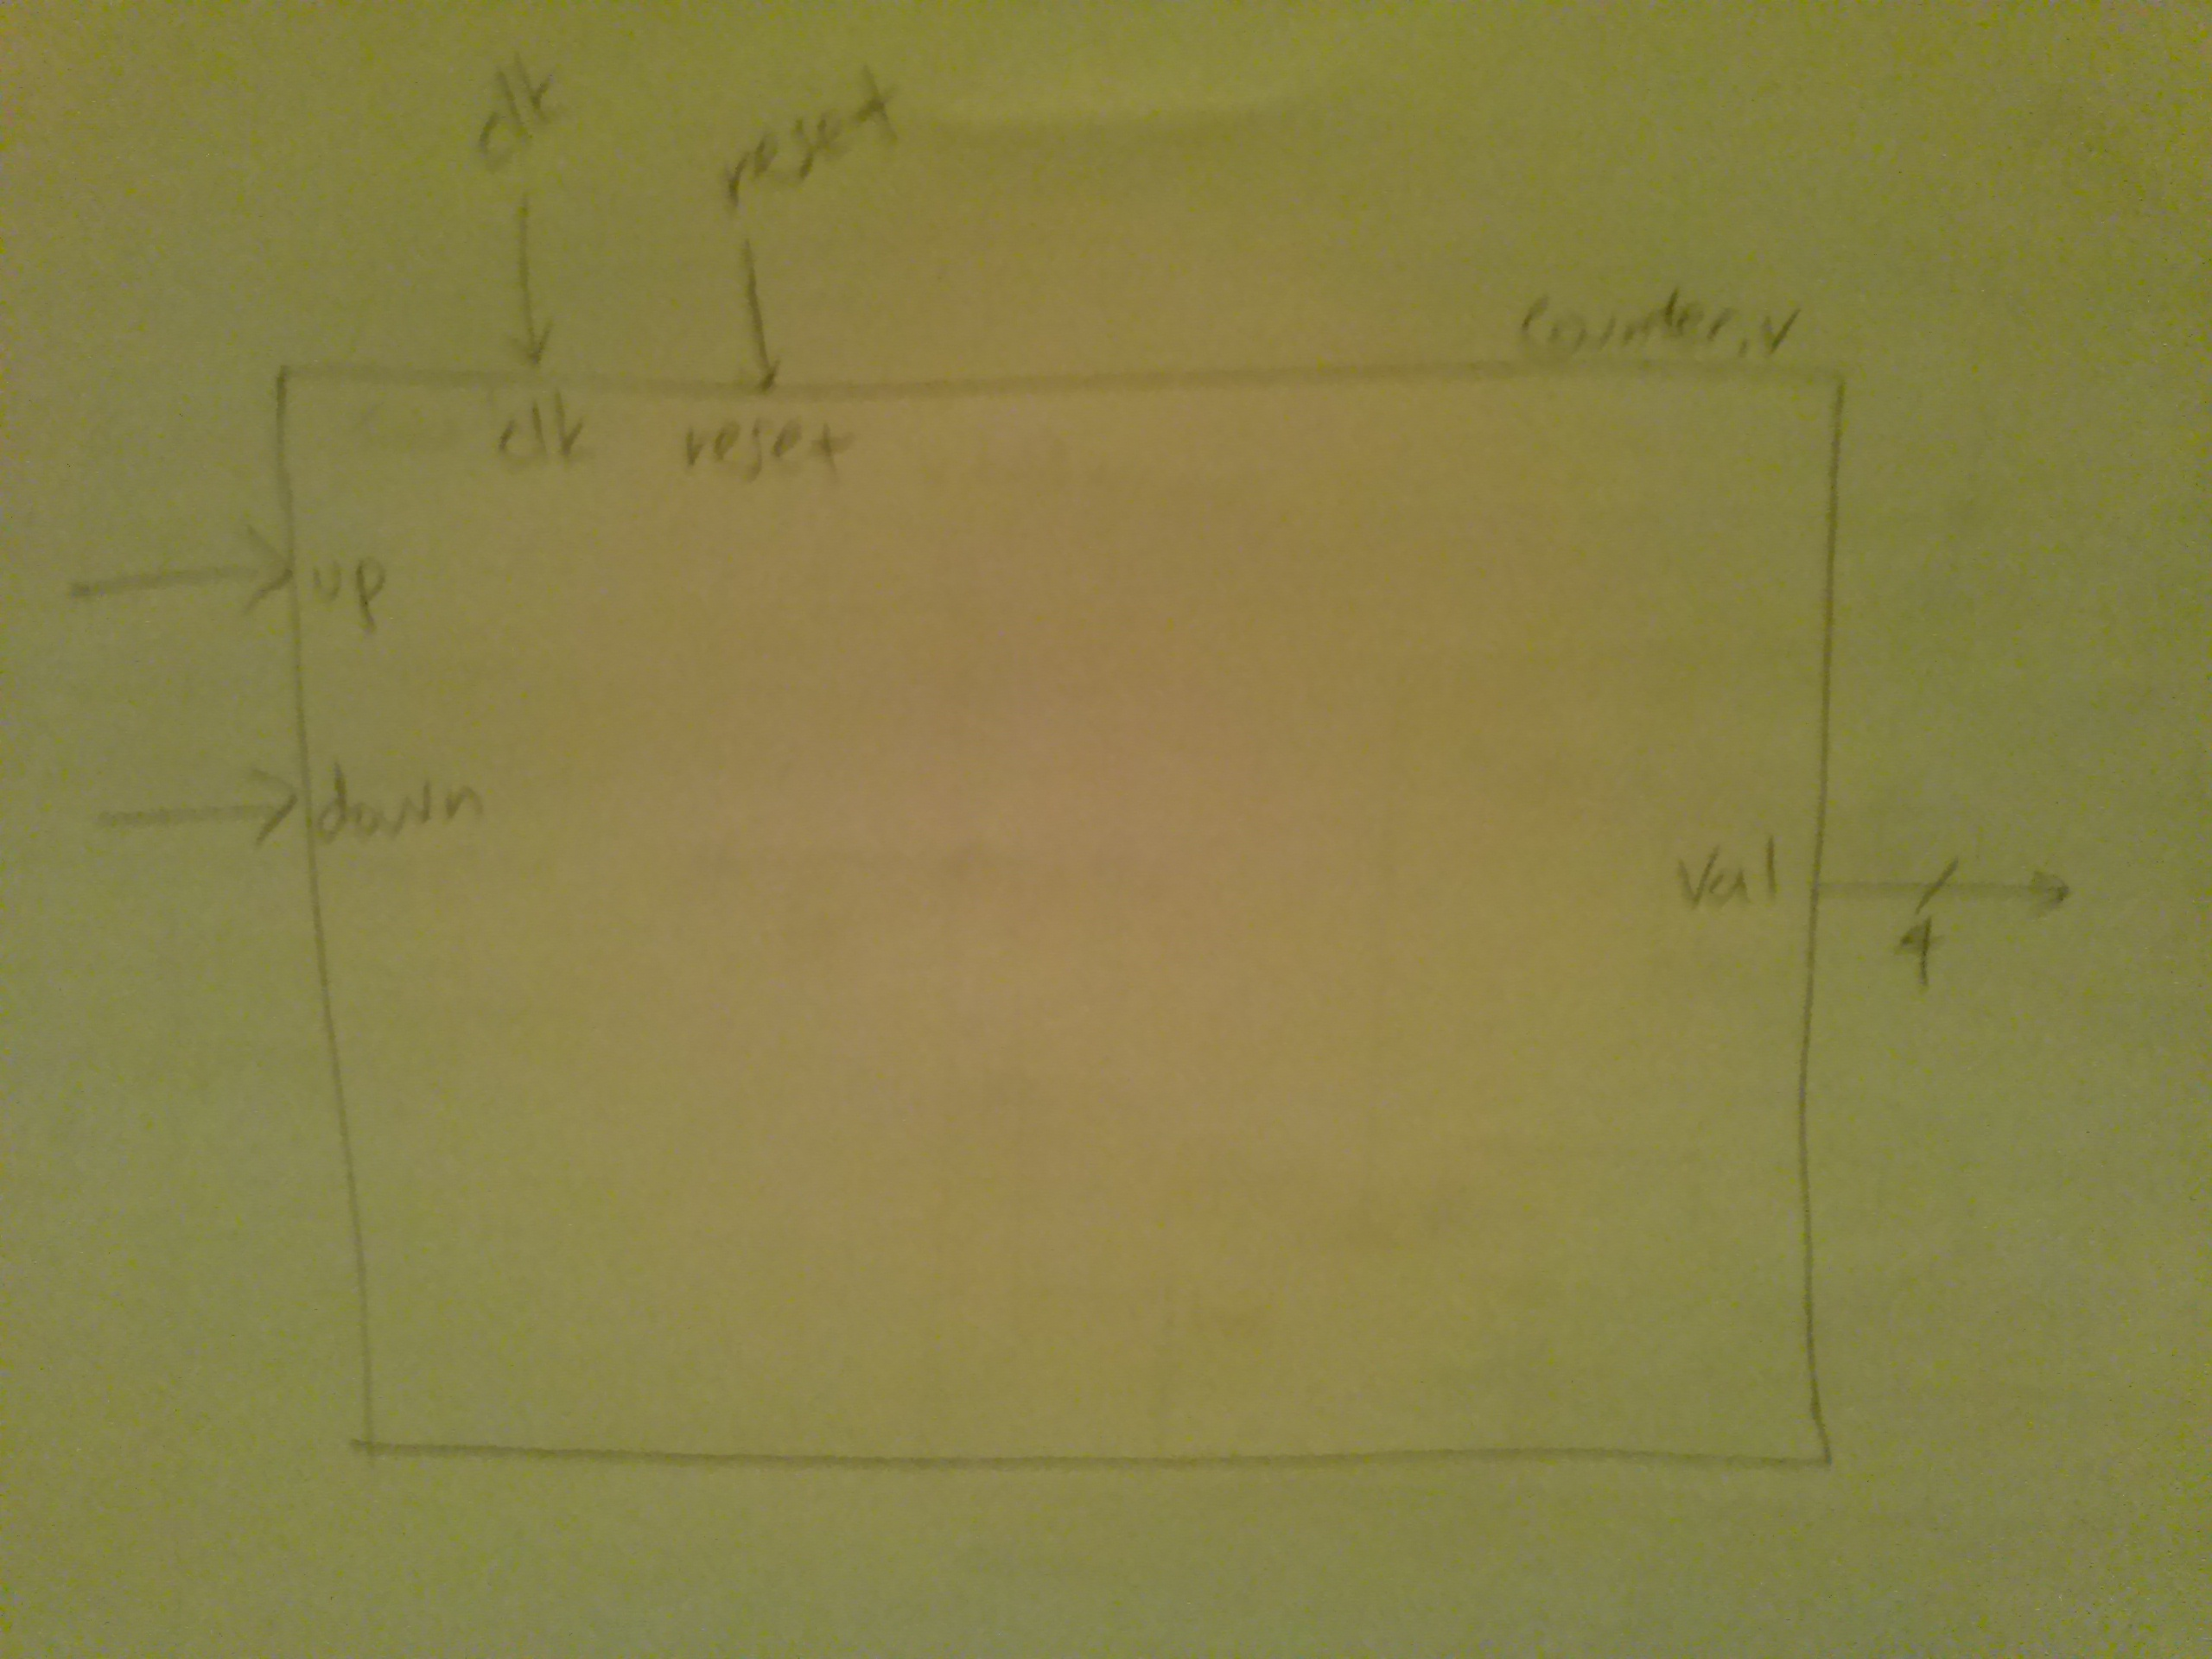
\includegraphics[width=0.75\linewidth]{figures/block_diagrams/counter.jpg}
        \caption{counter module block diagram}
        \label{fig:counter_blockdiagram}
      \end{figure}

      \begin{figure}[H]
        \centering
        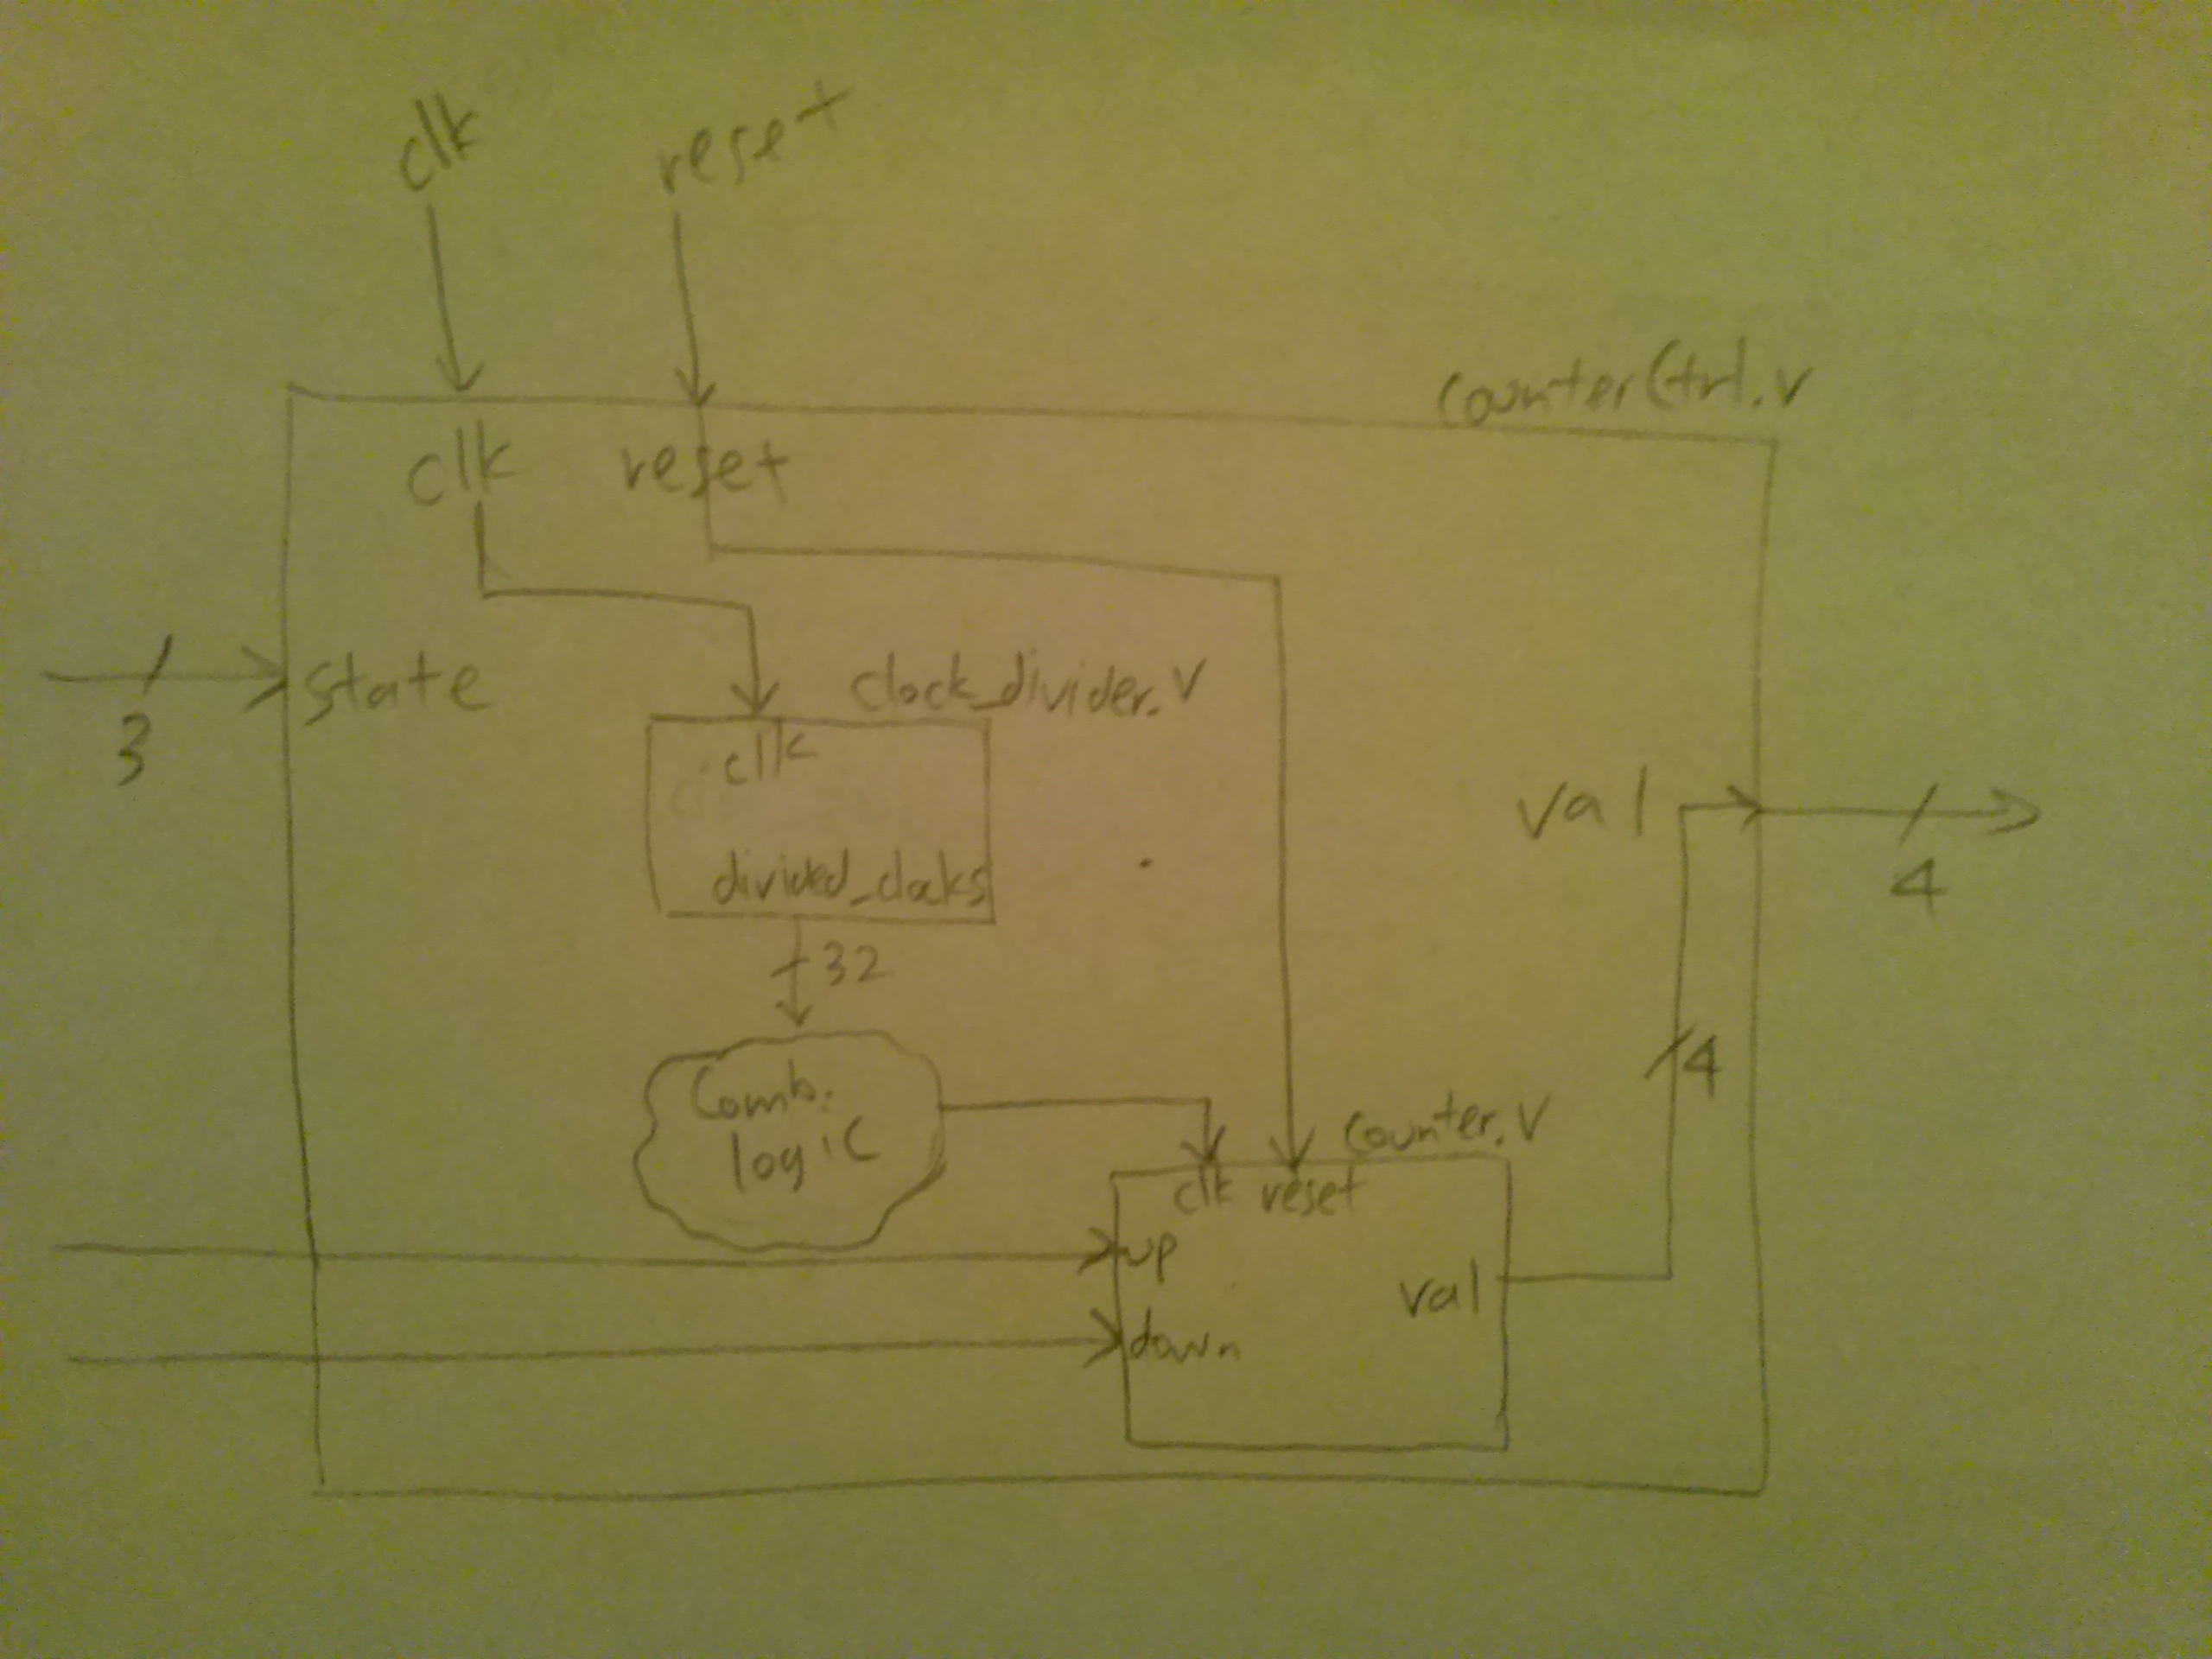
\includegraphics[width=0.75\linewidth]{figures/block_diagrams/counterCtrl.jpg}
        \caption{counterCtrl module block diagram}
        \label{fig:counterCtrl_blockdiagram}
      \end{figure}

      \begin{figure}[H]
        \centering
        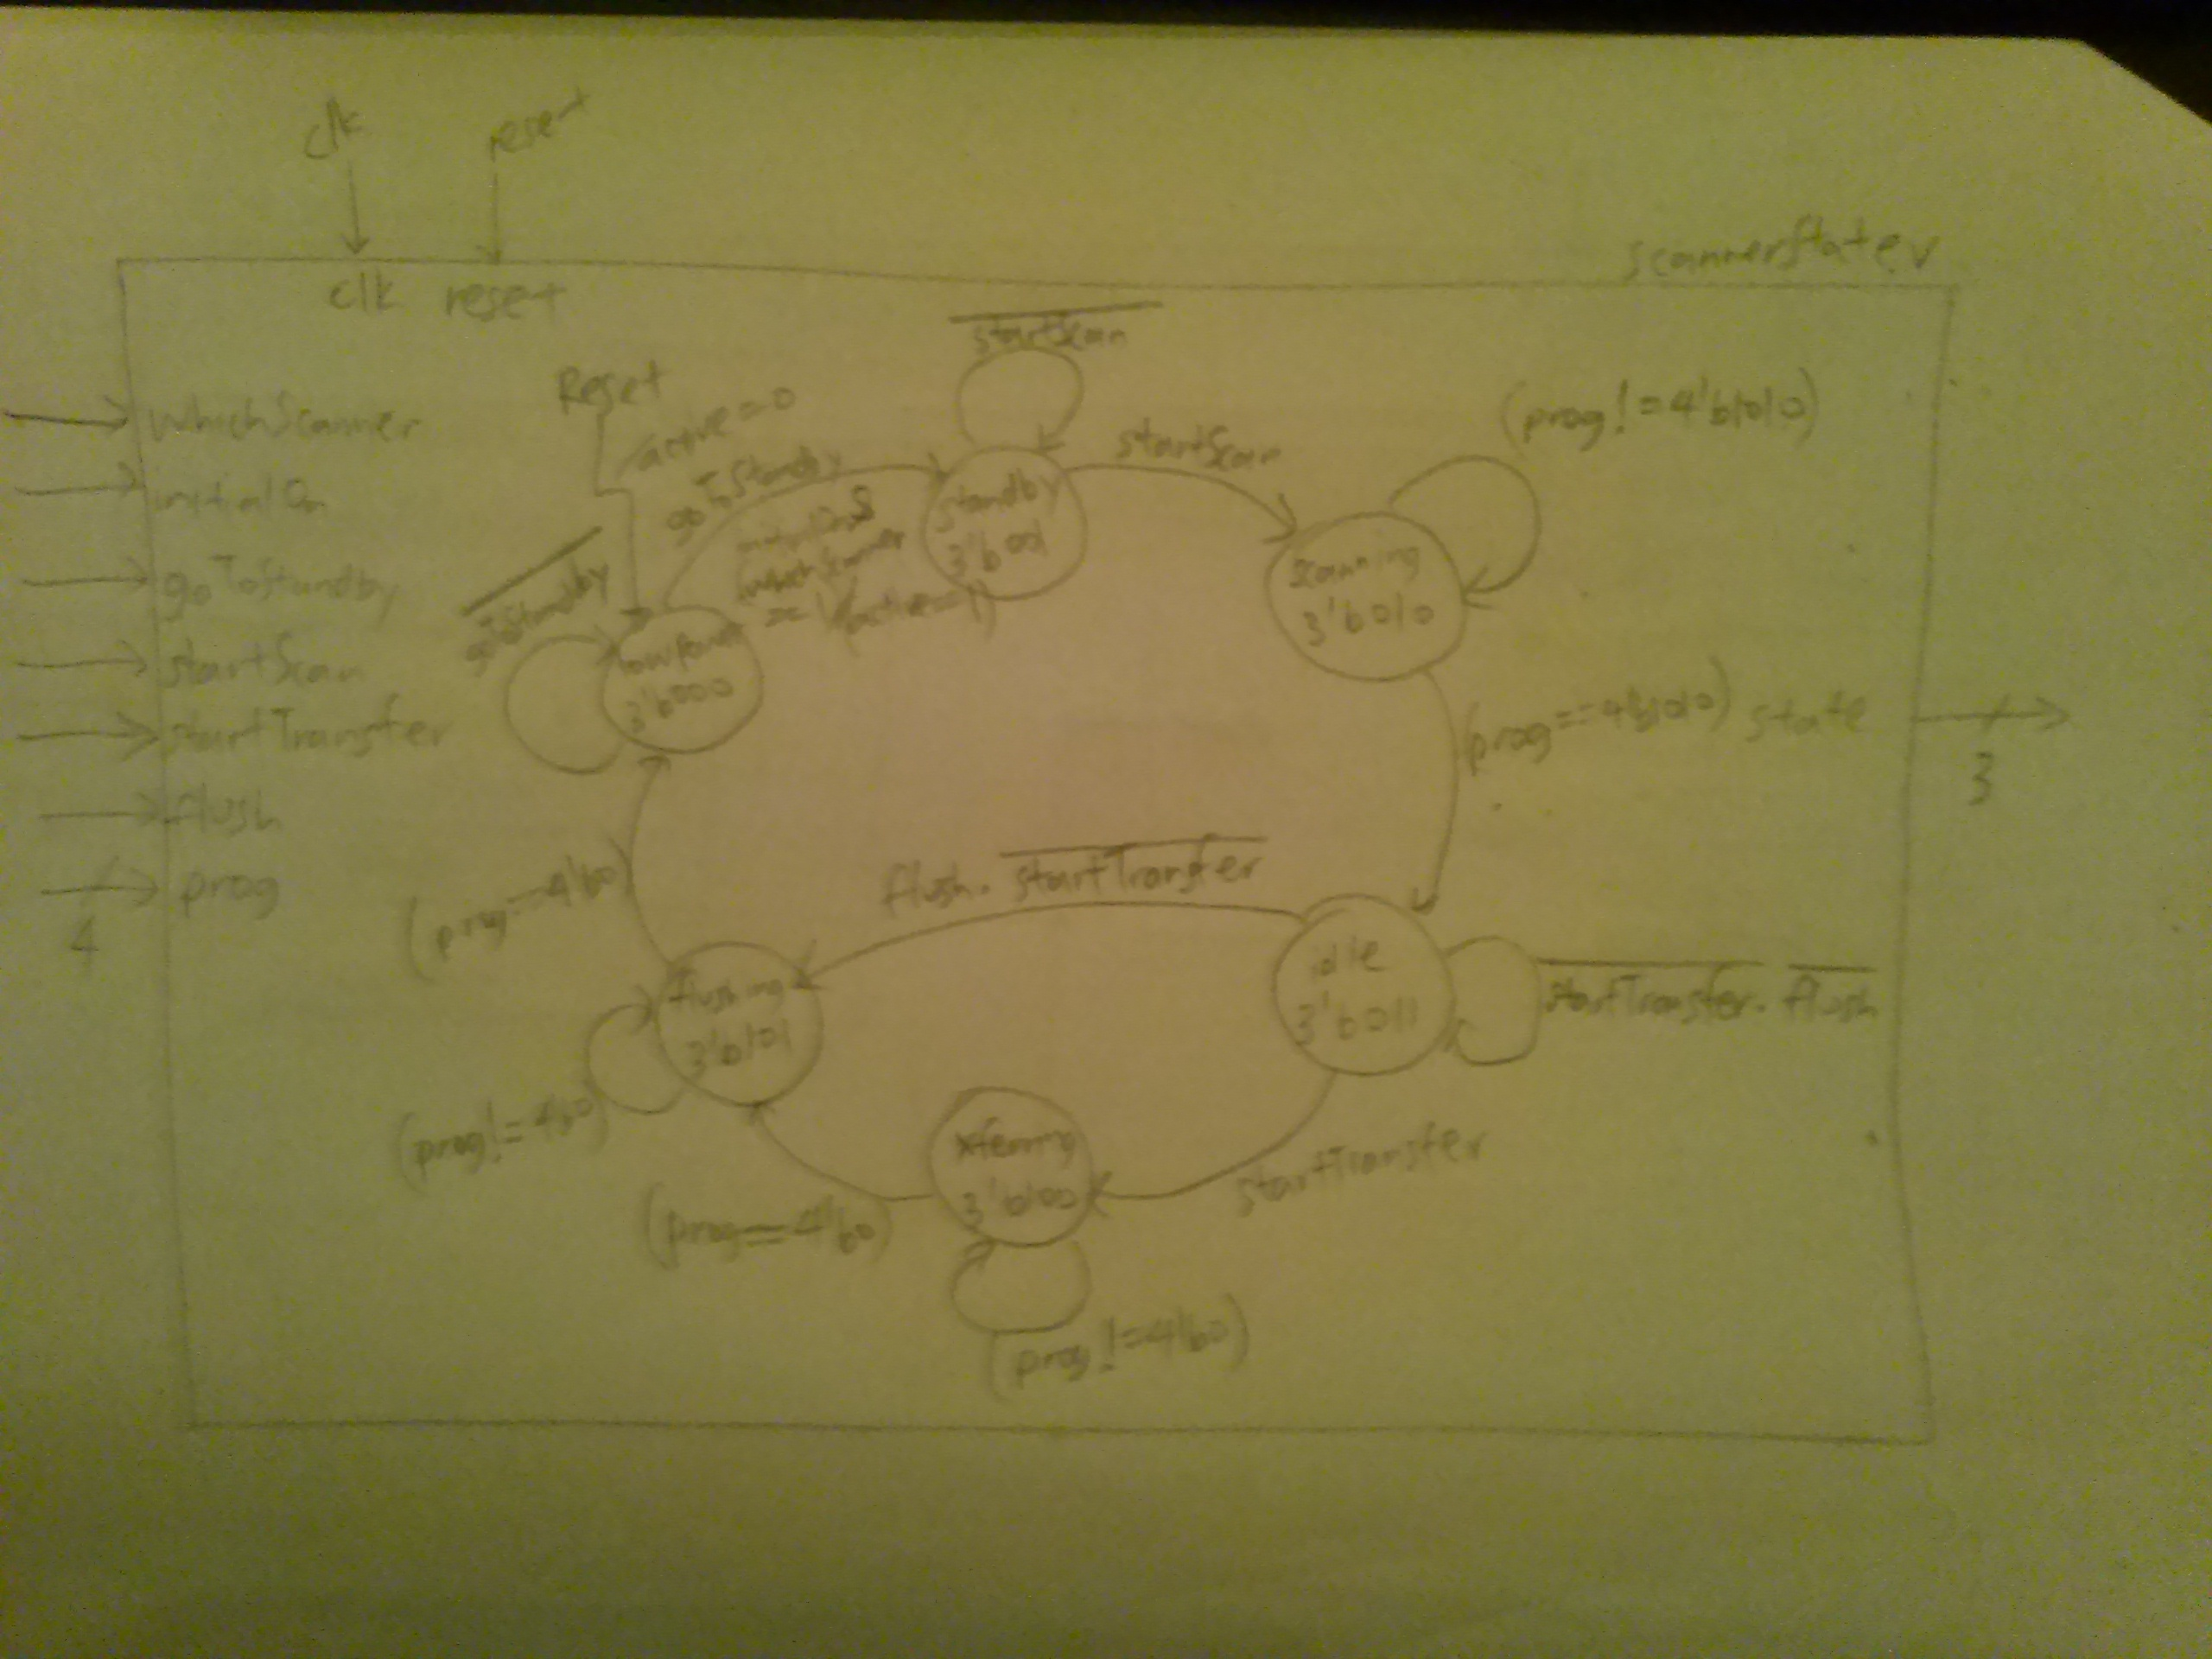
\includegraphics[width=0.75\linewidth]{figures/block_diagrams/scannerState.jpg}
        \caption{state transition diagram for the scanners}
        \label{fig:scannerState_FSM}
      \end{figure}

      \begin{figure}[H]
        \centering
        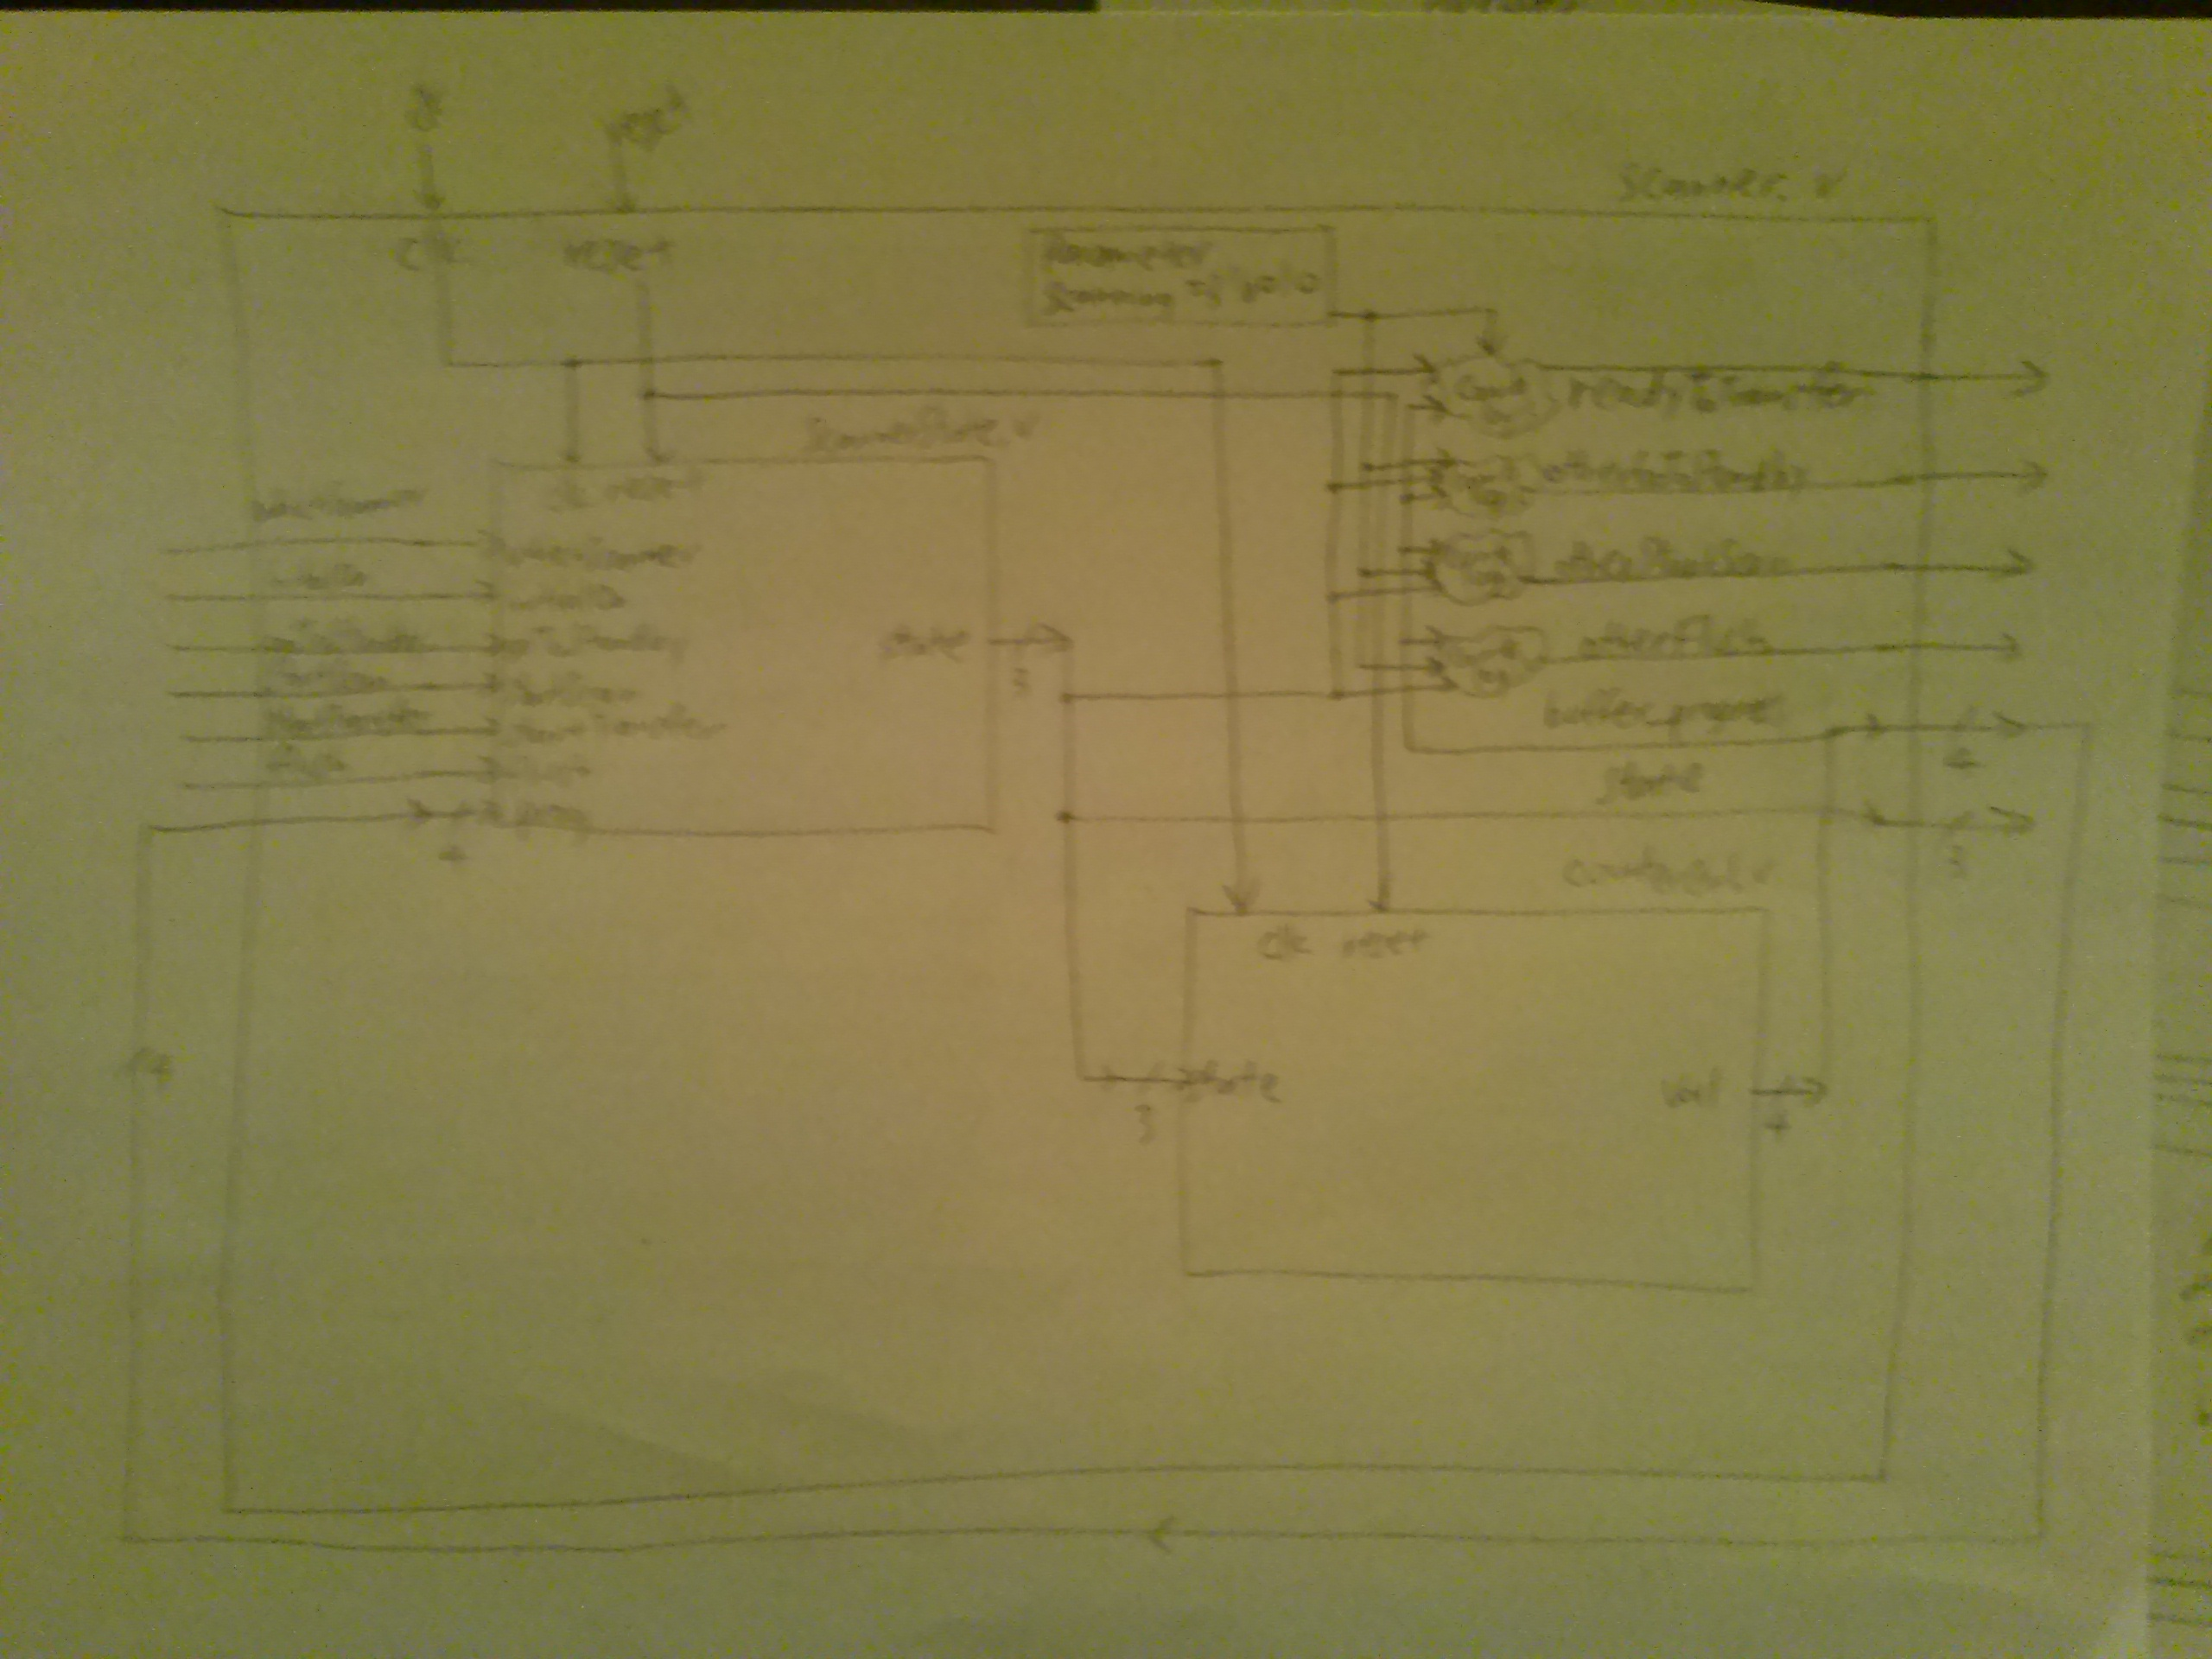
\includegraphics[width=0.75\linewidth]{figures/block_diagrams/scanner.jpg}
        \caption{scanner module block diagram}
        \label{fig:scanner_blockdiagram}
      \end{figure}

      \begin{figure}[H]
        \centering
        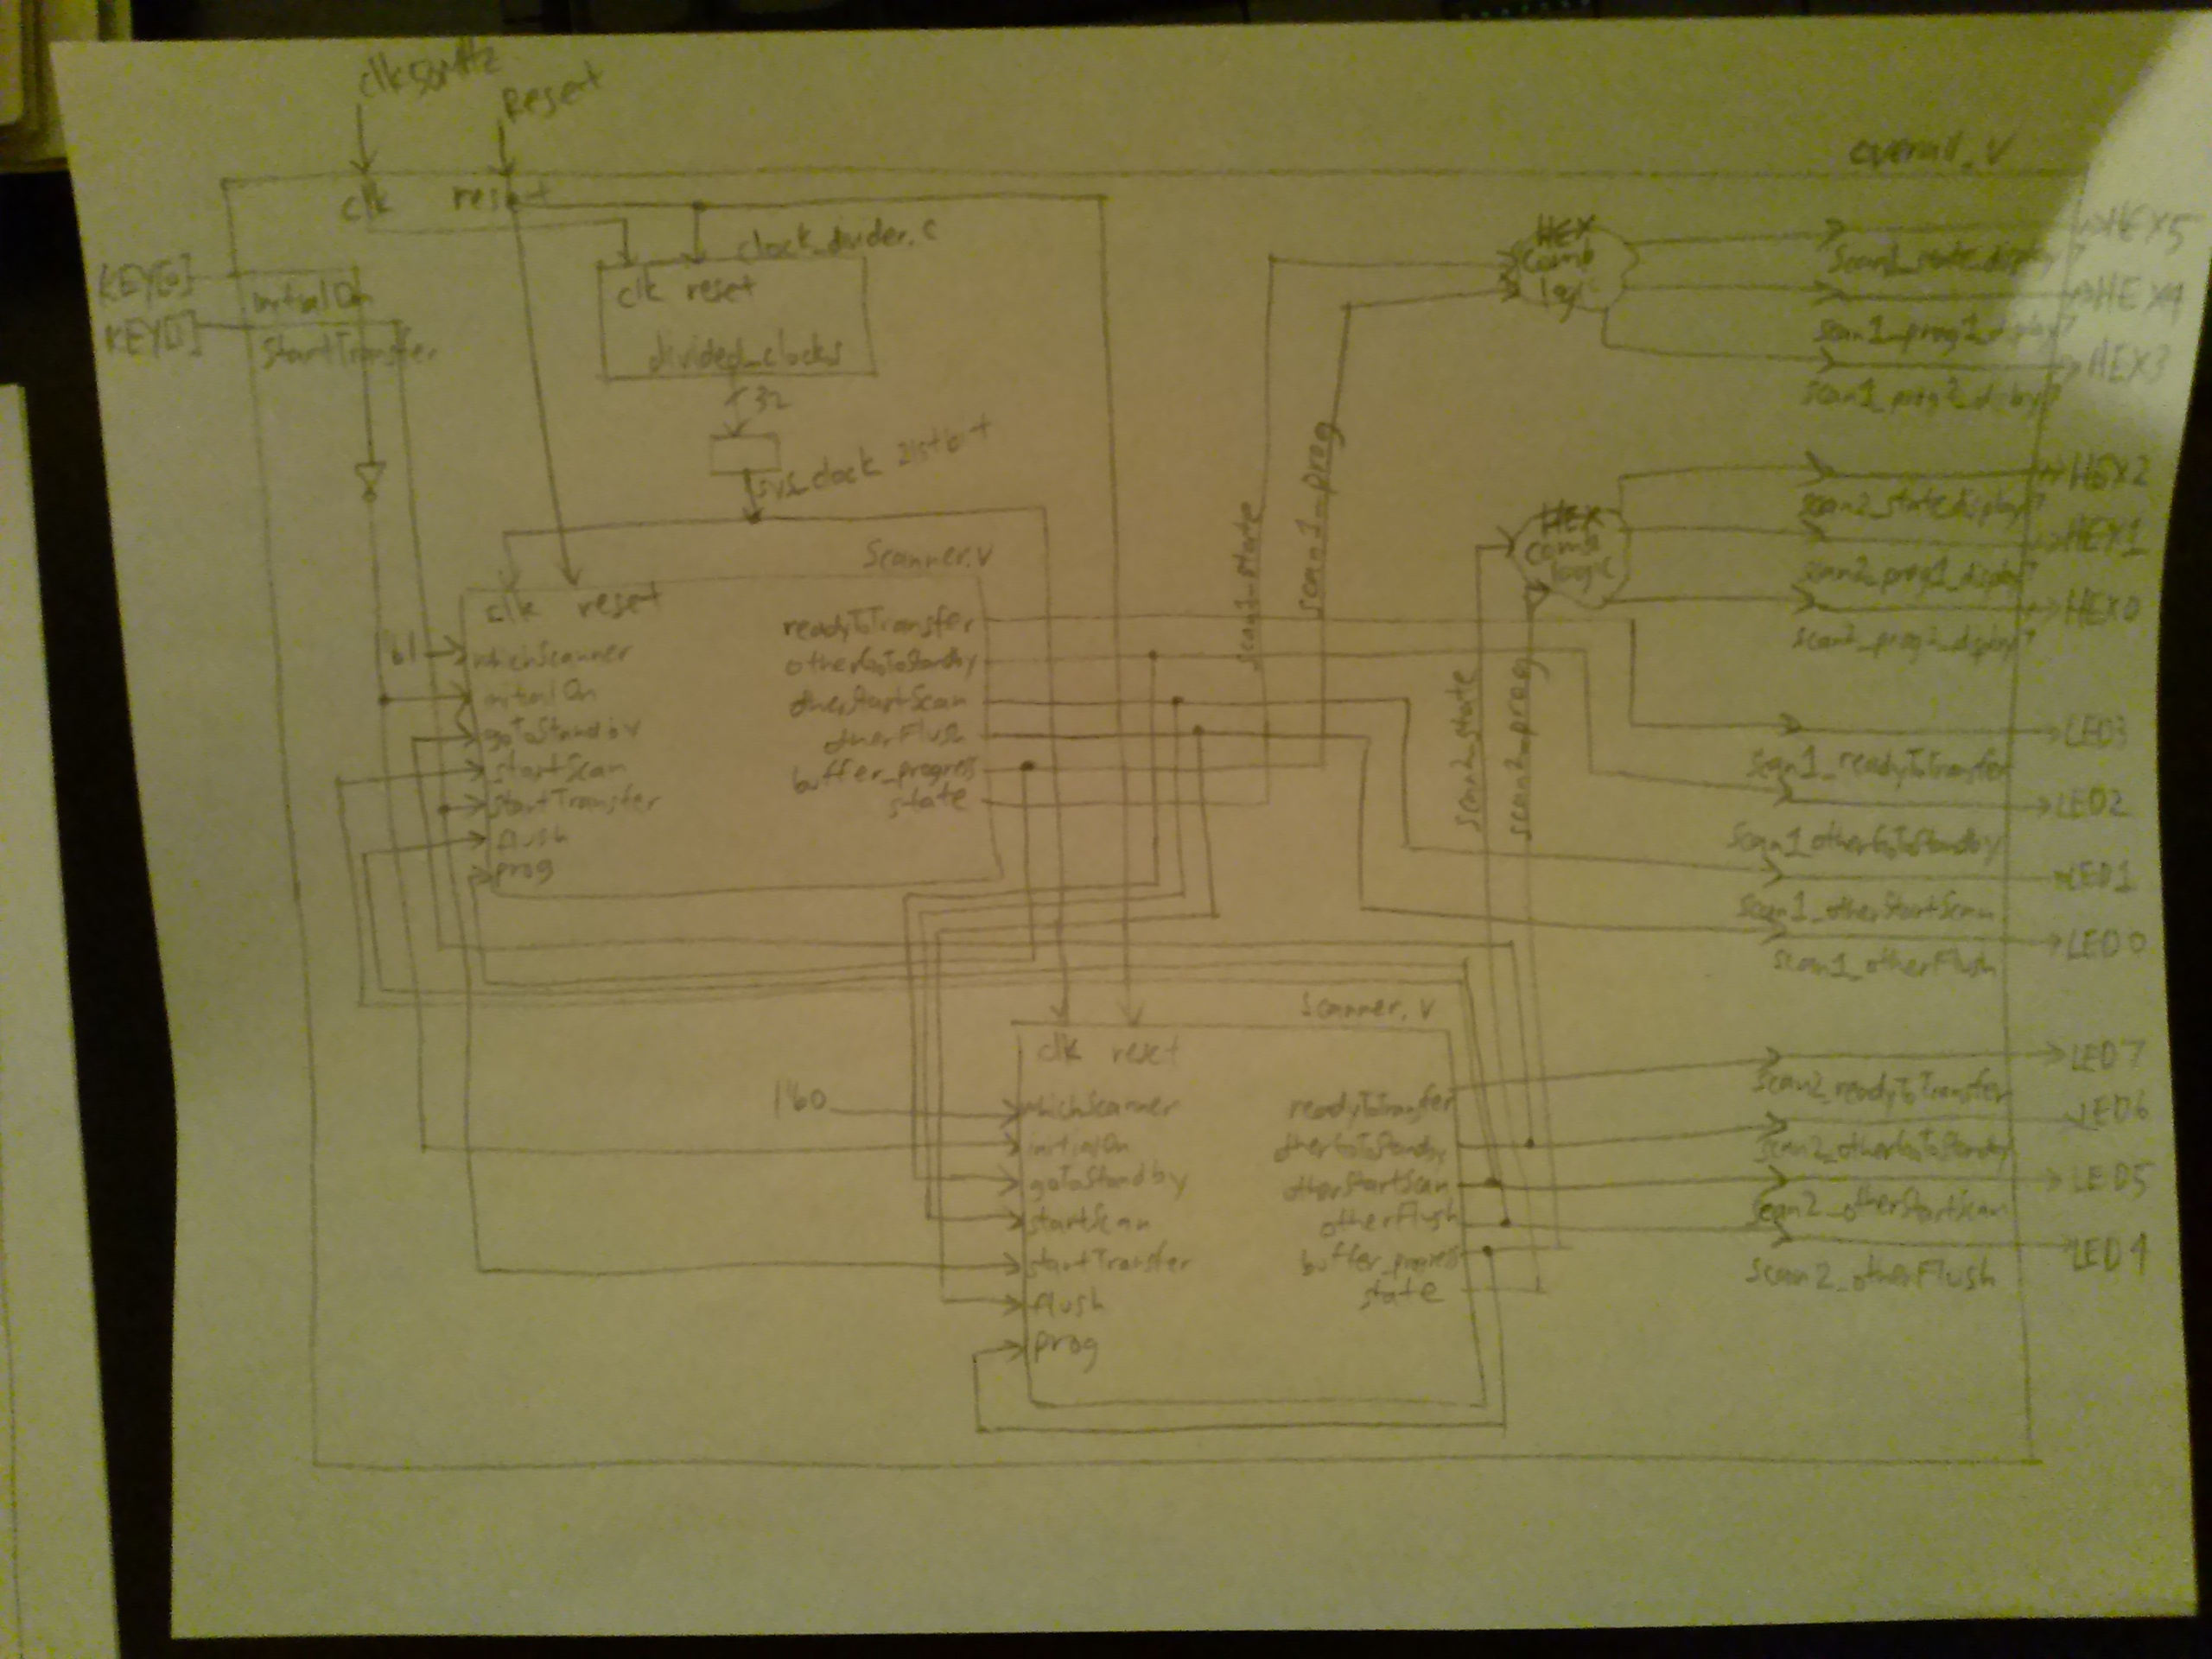
\includegraphics[width=0.75\linewidth]{figures/block_diagrams/overall.jpg}
        \caption{overall module block diagram}
        \label{fig:overall_blockdiagram}
      \end{figure}

    \subsubsection{Verilog code}
      % counter.v
      \lstinputlisting[language=Verilog]{../verilog/counter.v}
      \lstinputlisting[language=Verilog]{../verilog/counter_testbench.v}

      % counterCtrl.v
      \lstinputlisting[language=Verilog]{../verilog/counterCtrl.v}
      \lstinputlisting[language=Verilog]{../verilog/counterCtrl_testbench.v}

      % scannerState.v
      \lstinputlisting[language=Verilog]{../verilog/scannerState.v}
      \lstinputlisting[language=Verilog]{../verilog/scannerState_testbench.v}

      % scanner.v
      \lstinputlisting[language=Verilog]{../verilog/scanner.v}
      \lstinputlisting[language=Verilog]{../verilog/scanner_testbench.v}

      % overall.v
      \lstinputlisting[language=Verilog]{../verilog/overall.v}
      \lstinputlisting[language=Verilog]{../verilog/overall_testbench.v}

    \subsubsection{iverilog \& gtkwave waveforms}
      % counter gtkwave
      \begin{figure}[H]
        \centering
        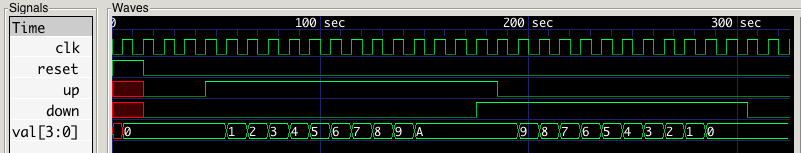
\includegraphics[width=0.75\linewidth]{figures/gtkwave/counter_gtkwave.png}
        \caption{counter module waveform}
        \label{fig:counter_gtkwave}
      \end{figure}

      % counterCtrl gtkwave
      \begin{figure}[H]
        \centering
        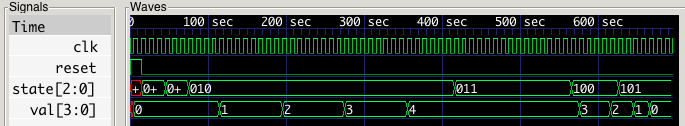
\includegraphics[width=0.75\linewidth]{figures/gtkwave/counterCtrl_gtkwave.png}
        \caption{counterCtrl module waveform}
        \label{fig:counterCtrl_gtkwave}
      \end{figure}

      % scannerState gtkwave
      \begin{figure}[H]
        \centering
        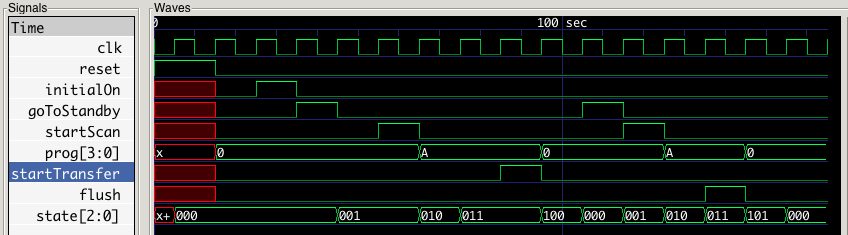
\includegraphics[width=0.75\linewidth]{figures/gtkwave/scannerState_gtkwave.png}
        \caption{scannerState module waveform}
        \label{fig:scannerState_gtkwave}
      \end{figure}

      % scanner gtkwave
      \begin{figure}[H]
        \centering
        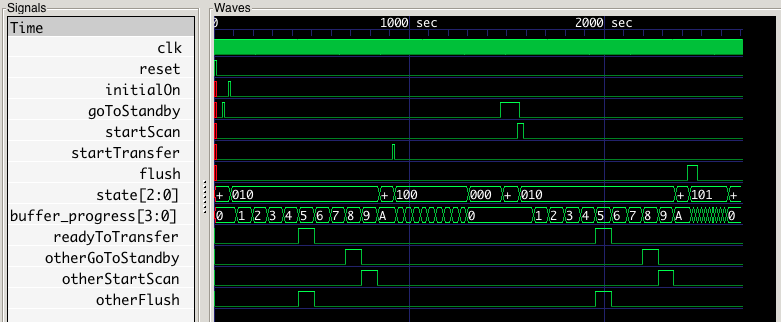
\includegraphics[width=0.75\linewidth]{figures/gtkwave/scanner_gtkwave.png}
        \caption{scanner module waveform}
        \label{fig:scanner_gtkwave}
      \end{figure}

      % overall gtkwave
      \begin{figure}[H]
        \centering
        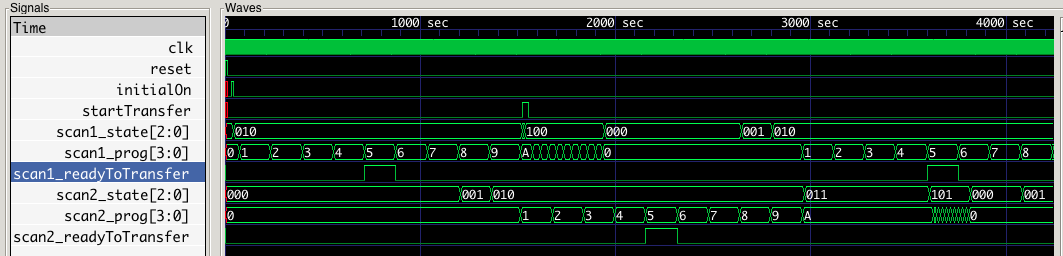
\includegraphics[width=0.75\linewidth]{figures/gtkwave/overall_gtkwave.png}
        \caption{overall module waveform}
        \label{fig:overall_gtkwave}
      \end{figure}

    \subsubsection{Signal Tap II data}
      \begin{figure}[H]
        \centering
        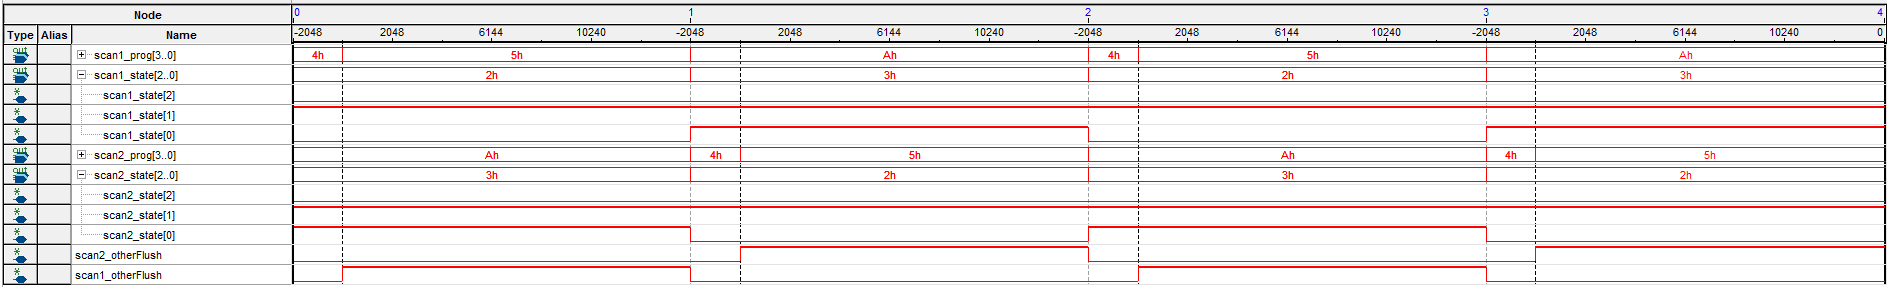
\includegraphics[width=0.75\linewidth]{figures/stp/flush_stp_output.PNG}
        \caption{SignalTap II data for flushing the scanners}
        \label{fig:flush_stp}
      \end{figure}

      \begin{figure}[H]
        \centering
        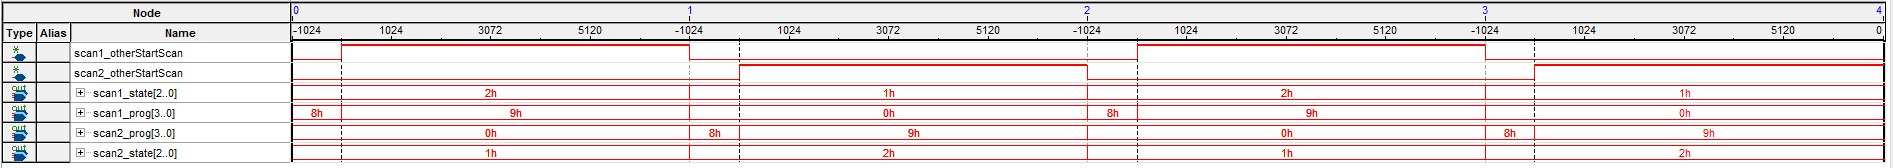
\includegraphics[width=0.75\linewidth]{figures/stp/startScan_stp_output.PNG}
        \caption{SignalTap II data for starting scanning}
        \label{fig:startScan_stp}
      \end{figure}

  \subsection{C Program}
    \lstinputlisting[language=C]{../c/calculateDelay.c}
    \lstinputlisting[language=C]{../c/temperature.c}

    % C program output
    \begin{figure}[H]
      \centering
      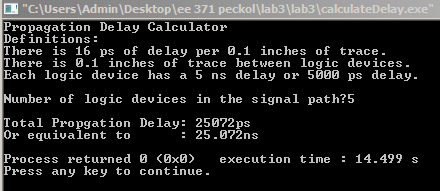
\includegraphics[width=0.75\linewidth]{figures/c/calc_normal.png}
      \caption{Normal output of calculateDelay program}
      \label{fig:calculateDelay_normal}
    \end{figure}

    \begin{figure}[H]
      \centering
      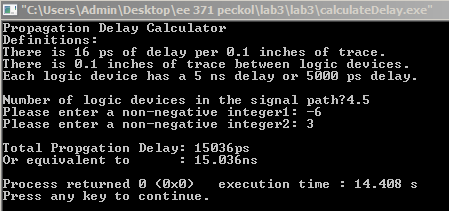
\includegraphics[width=0.75\linewidth]{figures/c/calc_errorhandle.png}
      \caption{Error handling output of calculateDelay program}
      \label{fig:calculateDelay_errorhandling}
    \end{figure}

    \begin{figure}[H]
      \centering
      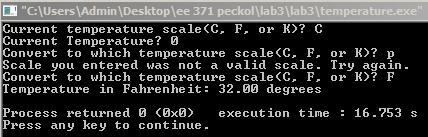
\includegraphics[width=0.75\linewidth]{figures/c/temp_CtoF.png}
      \caption{Output of temperature program: C to F}
      \label{fig:tempConv_CtoF}
    \end{figure}

    \begin{figure}[H]
      \centering
      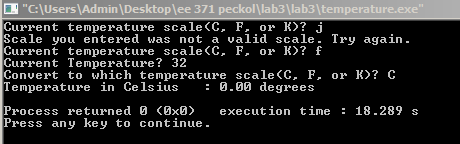
\includegraphics[width=0.75\linewidth]{figures/c/temp_FtoC.png}
      \caption{Output of temperature program: F to C}
      \label{fig:tempConv_FtoC}
    \end{figure}

    \begin{figure}[H]
      \centering
      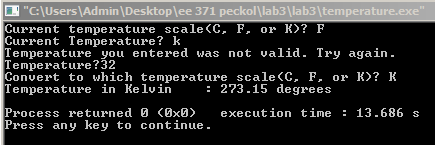
\includegraphics[width=0.75\linewidth]{figures/c/temp_FtoK.png}
      \caption{Output of temperature program: F to K}
      \label{fig:tempConv_FtoK}
    \end{figure}

    \begin{figure}[H]
      \centering
      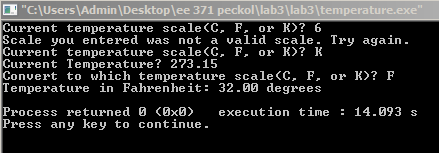
\includegraphics[width=0.75\linewidth]{figures/c/temp_KtoF.png}
      \caption{Output of temperature program: K to F}
      \label{fig:tempConv_KtoF}
    \end{figure}
\end{document}